\chapter{Higgs Boson Decay to Two Photons}
\label{chap:hgg}

The two photon channel is one of the most promising decay modes in 
the search for the SM Higgs boson at the LHC. 
Despite having a relatively small branching ratio, the decay $\Hgg$ 
provides a very clean final state in which the kinematics of the Higgs boson are 
fully reconstructed. It is, therefore,
one of the most sensitive channels at low $\mh$.
The dominant source of background is from real, prompt diphoton events from QCD 
processes, $pp\rightarrow\gamma\gamma$ (prompt-prompt).
In addition, there are contributions from $pp\rightarrow\gamma+jet$ (prompt-fake) and 
$pp\rightarrow jet+jet$ (fake-fake) in which jets are misidentified as photons. 
In high-priority analyses such as the search for the Higgs boson, cross-checking of analysis
techniques is essential to ensure a robust result. At CMS, it is the policy to design at least two 
different techniques for the same analysis ideally implemented in independent code bases.
In particular, as the signal rate in the $\Hgg$ decay mode is small compared to the background rates,
the sensitivity of the search is heavily influenced by how well the backgrounds are understood.
For these reasons, two data-driven techniques for extracting the signal were developed.
The first (method A) uses a fully parametric description of the background which is fitted to the data. 
The type of parameterisation and the number of parameters are chosen so that the systematic uncertainty 
introduced by potentially choosing the wrong functional form is less than $\frac{\displaystyle 1}{\displaystyle 5}$ 
of the statistical uncertainty in the fit~\citep{HIG-11-033}.
The second (method B) uses a binned model constructed from 
sidebands in the diphoton invariant mass spectrum. 
Method B was developed by the author and serves as an independent 
cross-check of method A. In particular, this is achieved by allowing direct 
inclusion of the background modelling systematic uncertainties in the signal extraction, thereby building 
confidence in the understanding of the background. 
This chapter describes a search for a Higgs boson decaying to two photons
which was performed on the full 2011 dataset corresponding to \clumi of proton-proton collisions 
recorded at CMS at a center of mass energy of 7 TeV.
In Sections~\ref{sec:datasamples} to~\ref{sec:eventselection}, the reconstruction and
selection of events used for this analysis is detailed. Section~\ref{sec:signalextraction} 
then describes method B for modelling the background for the purposes
of extracting a potential signal and statistical interpretations of the data. 
%Figure~\ref{fig:mvaoverview} is a flow chart of the analysis strategy indicating the point 
%at which the two methods diverge. 
Results from the 2011 dataset are given in Section~\ref{sec:hggresults2011} and the update for the ICHEP conference in July 2012
at which the discovery announcement of the new boson was made is given in~\ref{sec:8tev}.

\begin{figure}
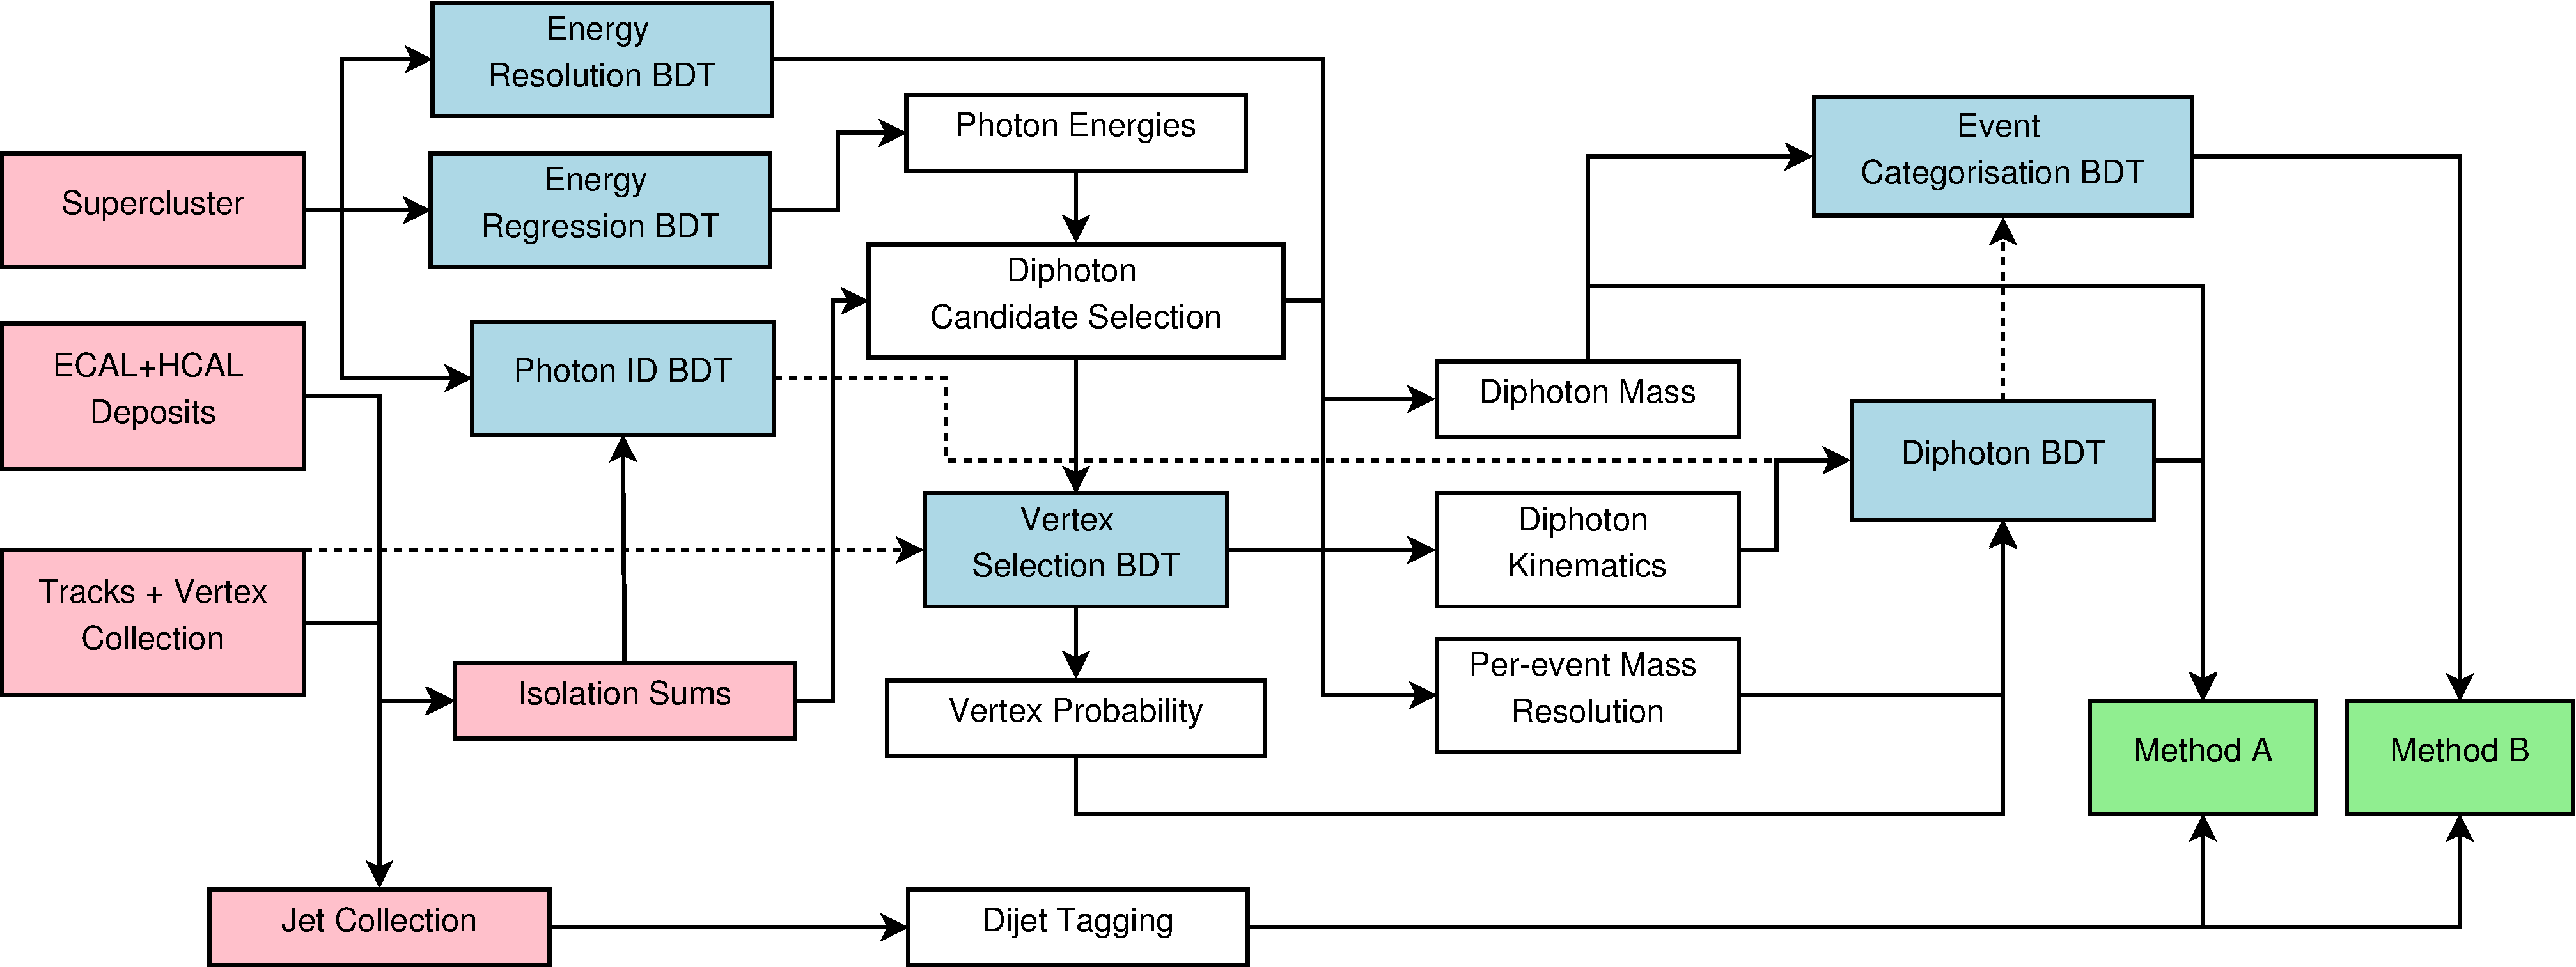
\includegraphics[width=\textwidth]{hgg7TeV/generalPlots/mvaflowchart.pdf}
\caption{Flow chart of the $\Hgg$ analysis performed on the 2011 dataset. The blue boxes
 indicate stages which involve the use of a boosted decision tree (BDT). The red boxes indicate 
inputs from the common CMS reconstruction and are not detailed in this chapter. The two 
methods for signal extraction, labelled A and B, are indicated by the green boxes.}
\label{fig:mvaoverview}
\end{figure}

\section{Data Samples}
\label{sec:datasamples}

The dataset used for this analysis is taken from a combination of the 2011A 
(March-August) and 2011B (September-October) proton-proton collision runs.
The selection of the dataset is based around dedicated diphoton triggers
which select events satisfying one of two sets of criteria.
The first set requires two HLT photon candidates, one with $\pt>26$ GeV and the other with 
$\pt>18$ GeV, which are well isolated in the calorimeter~\citep{AN-12-048}. The second has a lower threshold on
the first photon, $\pt>22$ GeV but requires that both photons have localised showers in the ECAL 
($\rnine>0.8$ in 2011A and $\rnine>0.9$ in 2011B). 
Additionally, the invariant mass of the two trigger objects is required to be 
greater than 60 (70) GeV in the 2011A(B) datasets.
Events which would pass the full offline selection but fail to trigger at the HLT lead to an inefficiency, 
reducing the number of signal events with respect to that expected from an integrated luminosity of \clumi.
However, the thresholds applied offline are chosen to be much tighter than those of the trigger;
the trigger efficiency is $>$99\% with respect to the analysis selection~\citep{AN-12-048}. 

Signal Monte Carlo (MC) events are generated for a Higgs boson decaying to two photons via the four main 
production processes, gluon-gluon fusion ($ggH$), vector boson fusion ($qqH$) and associated $W/Z$ ($VH$) 
and $\ttbar$ ($ttH$) production.
The gluon-gluon fusion and vector boson fusion processes were generated with \texttt{POWHEG}~\citep{powheg} with 
next-to leading order (NLO) contributions whereas
the two associated production processes were generated to leading order (LO) only.
The $\pt$ spectrum of the Higgs boson ($\pt^{H}$) from gluon-gluon fusion was calculated at
next-to-next-to leading plus next-to leading log resummed order (NNLO+NLL) using the \texttt{HqT} program~\citep{hqt}.
The production cross-sections and branching ratios are taken from the LHC Cross-section Working Group~\citep{lhcxswg}.

Background processes were generated at LO using \texttt{POWHEG} interfaced with \texttt{PYTHIA}~\citep{pythia}.
The QCD dijet and $\gamma+jet$ samples were filtered by requiring the generated photons, electrons and neutral
mesons with $\pt>15$ GeV have at most one charged particle in a cone, $\Delta R<0.2$, to increase the 
production efficiency with respect to the tracker isolation requirements of the full selection.
The background samples considered for this analysis are summarized in Table~\ref{tab:backgroundmc}.
A full simulation of the CMS detector is provided in \texttt{GEANT4} which is used for all signal
and background MC samples~\citep{geant4}. The MC includes a simulation of additional interaction vertices expected in data
from pileup. This is where multiple pp collisions occur within a single bunch crossing which results in several
primary vertices being reconstructed. The distribution in the number of reconstructed vertices in 
MC is corrected to match that observed in data.

\begin{table}
\begin{tabular}{|l r|c|c|}
\hline
\textbf{Process}  & &  \textbf{Cross-section} ($pb$) & \textbf{Luminosity} ($pb^{-1}$)\\
\hline
\hline
DiPhotonJets & & 154.7 & 7400 \\
\hline
DiPhoton Box & $\hat{\pt}~25-250$ & 12.37 & 41900 \\
\hline 
QCD Dijet    & $\hat{\pt}~30-40$      & 10870 & 560 \\
	     & $\hat{\pt}~40-\infty$  & 43571 & 920 \\
\hline 
Gamma+Jet    & $\hat{\pt}~20-\infty$  & 493.44& 2400 \\
\hline 
DrellYan+Jets to $ll$  & $\hat{\pt}~50-\infty$  & 2475& 14000 \\
\hline
\end{tabular}
\caption{Background MC used throughout the analysis with production cross-sections and 
corresponding equivalent integrated luminosity. The prompt-prompt ($\gamma\gamma$) sample 
comprises events from the DiphotonJets and Diphoton Box samples. Both the QCD dijet and Gamma+Jet
 contain prompt-fake ($\gamma j$) events. The samples are filtered to avoid double counting
of this background. Fake-fake ($jj$) events are taken from the QCD Dijet sample.}
\label{tab:backgroundmc}
\end{table}

\section{Object Reconstruction and Identification}
\label{sec:objectrecoandid}

The reconstruction of all objects used for this analysis, in both data and MC,
is based on the standard CMS reconstruction software \texttt{\cmssw}~\citep{cmssw}. 
Additional sensitivity can be gained by refining the object selection and reconstruction specifically
to the search for $\Hgg$.

\subsection{Boosted Decision Trees}
\label{sec:bdts}
Multivariate analysis (MVA) techniques are often used in high energy physics analyses
which suffer from the presence of large background rates. These techniques provide
greater distinction between signal and background than traditional selection 
techniques. This is due to the fact that the full information from each event 
can be utilised by describing the event with a set of measurable quantities. 
The distributions of these quantities and correlations between them can be 
exploited to provide the maximum separation between signal and background.
Of the many MVA techniques available, Boosted Decision Trees (BDT) are commonly used 
in high energy physics as they are robust against the inclusion of non-informative variables; 
the performance will not degrade due to the addition of information which offers little or no 
separation power~\citep{tmva}.
 

BDTs are used in the $\Hgg$ search described in this
chapter in order to achieve the maximum sensitivity to a potential signal.
For most of the BDTs used in this analysis, the BDT is used to provide 
separation between signal and background processes. 
The first step in producing a BDT of this type is to identify a list of ``input'' 
variables which describe the event objects and provide discrimination 
between signal and background.  
These can be variables such as the $\rnine$ and $\sigieie$ 
of the photon superclusters or kinematic variables of the event such as
the transverse momentum of the diphoton system ($\ptgg$). 
Additional variables, such as the positions of the photons within the detector, 
are included so that the BDT can account for correlations between the 
input variables due to detector effects.

A decision tree (DT) is then trained on a MC simulation sample of signal and background 
events. The DT splits the events into two sub-samples by applying a series of cuts
on the input variables. The purity, $p$, of each sub-sample is defined as 
the fraction of the events which are signal, 
\begin{equation}
p = \frac{N_{s}}{N_{s}+N_{b}},
\end{equation}
where $N_{s}$ and $N_{b}$ are the sum of weights for the signal and background samples.
A separation criterion is defined to decide whether or not to further sub-divide
that subset. A number of criterion definitions exist, though commonly the 
Gini index~\citep{tmva}, $p(1-p)$ is used. Values which are close to one indicate 
the sample is polluted by background, so above some configurable threshold, 
the sub-sample is further split and the process continues. 
This continues until either all sub-samples are below the threshold or the
user-defined maximum number of splitting levels (tree depth) is reached. 
Each MC event is then assigned a value of -1 or +1 depending on whether it is
or is not in a sub-sample with $p>0.5$. The DT is trained by varying the cuts 
applied in order to maximise the purity in each sub-sample.
Several events will be incorrectly classified by simply taking the output of the DT.
This is mitigated by training a set of DTs on the same sample and modifying the 
contribution from each DT through a processes known as ``boosting''. 
A weight is applied simultaneously to all of the DTs by minimising the 
binomial log-likelihood loss function for the sample of $K$ events,
\begin{equation}
L(F,y) = \sum_{k=1}^{K} \ln\left(1+e^{-2 Fy} \right),
\end{equation}
where $y=-1$ for a background event and $y=+1$ for a signal event.
Each DT can be considered as a member of a family of functions $f(\mathbf{x};\mathbf{b}_{n})$ 
for a particular set of cut values $\mathbf{b}=\mathbf{b}_{n}$~\citep{friedmanbdt}.
The function $F$ is the weighted average over the individual DTs given by,
\begin{equation}
F(\mathbf{x};\mathbf{a},\mathbf{b}_{n}) = 
	\sum_{n=0}^{N}a_{n}f(\mathbf{x};\mathbf{b}_{n});~\mathbf{a}=(a_{1},a_{2}\cdots a_{N}).
\end{equation}
Although other weighting schemes can be used, for the BDTs trained in this analysis, 
the scheme described, known as gradient boosting, was found to give the best performance 
(see Section~\ref{sec:signalextraction}).
The resulting set of trees is known as a boosted decision tree. 
All of the BDTs used for this analysis were trained using the \texttt{TMVA} 
toolkit~\citep{tmva} available within the \texttt{ROOT} framework.
\subsection{Supercluster Energy Correction}
\label{sec:superclusterenergyreconstruction}

As the natural width of the Higgs boson is around 100 MeV at low $\mh$, 
the width of a reconstructed mass peak from 
a $\Hgg$ decay is driven by the experimental energy resolution of the photons.
This resolution can be improved dramatically by correcting the raw energy of the supercluster 
at the per-photon level. These corrections are derived using a multivariate technique 
in which a regression BDT is trained on prompt photons in the gamma+jet MC sample using the 
ratio of the generated photon energy to the raw energy of the reconstructed supercluster~\citep{AN-12-160}.
As this ratio can vary across different regions of the detector, 
the input variables include both the $\eta$ and $\phi$ positions of the supercluster.
In addition, several variables are included which describe the shower shape: $\rnine$, 
the energy weighted widths in $\eta$ and $\phi$ of the supercluster, the energy 
weighted crystal width ($\sigieie$) and the ratio of hadronic energy behind the supercluster
to the energy of the supercluster itself ($\hoe$). 
In the endcaps, there is additional information 
available from the pre-shower measurement so the ratio of the energy in 
the pre-shower to the raw supercluster energy is included. 
Figure~\ref{fig:mcregrcomparison} shows the improvement
in resolution after applying the regression corrections (Raw + Regression) compared to the standard 
calibrations used at CMS (Standard). In parallel, a similar set of corrections were derived by 
fitting an analytical expression (Standard + IC Residual) to the residual energy difference between the 
generated and reconstructed photon energy as a function of 
supercluster energy, position and $\rnine$~\citep{AN-11-343}. 
The regression technique reduces the effective resolution of the Higgs mass peak ($\sigma_{\mathrm{eff}}$) 
resolution by around 30\% over using the raw supercluster energy 
compared to the analytic fit which improves the resolution by 15\%. 

\begin{figure}
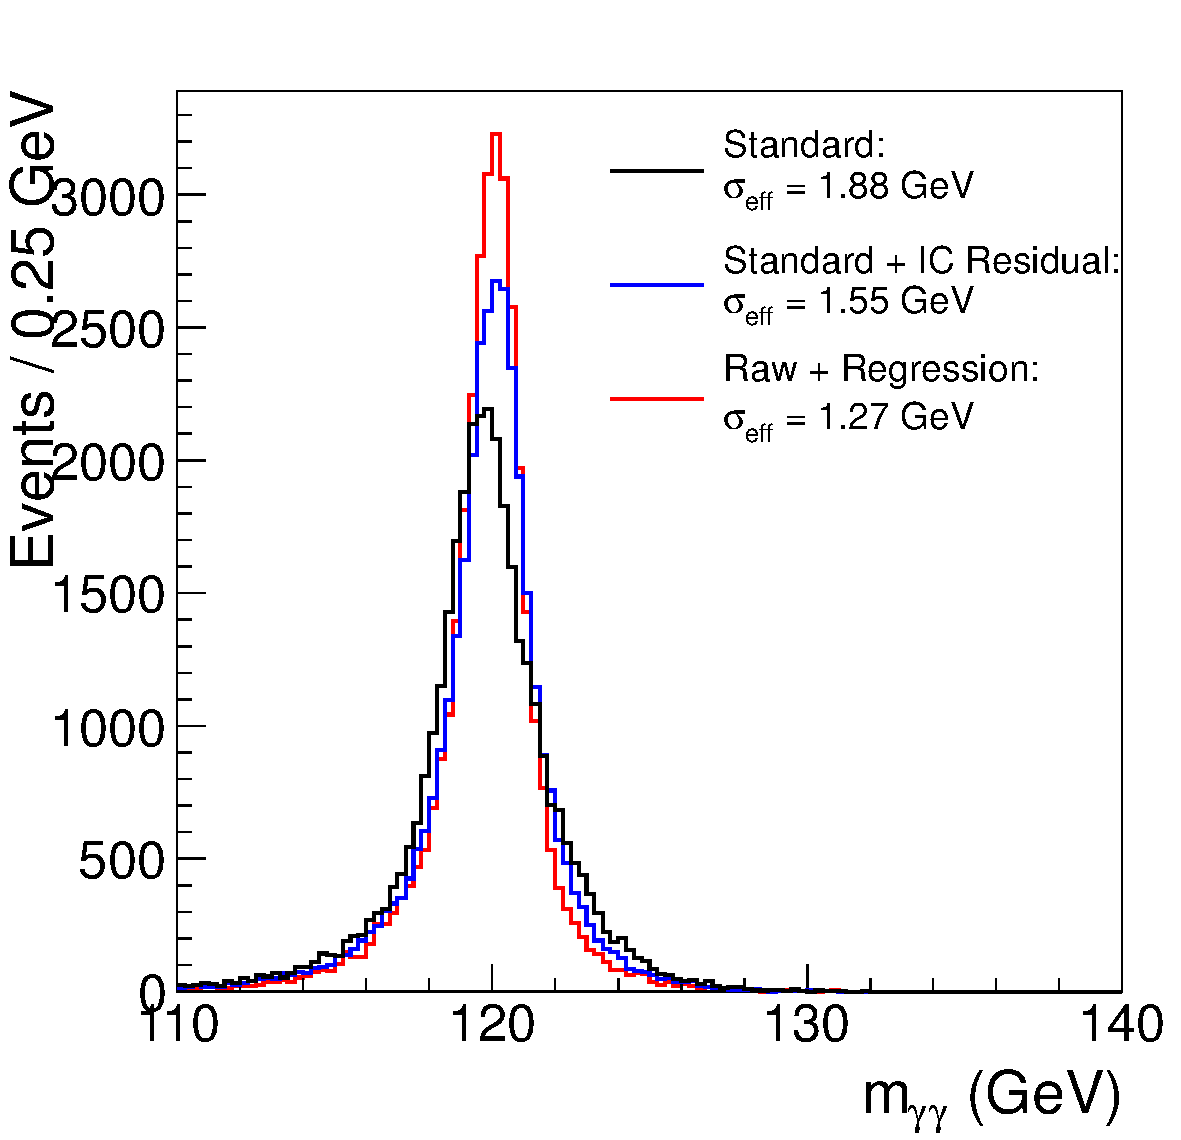
\includegraphics[width=.6\textwidth]{hgg7TeV/generalPlots/regrresall.pdf}
\caption{Comparison of the diphoton mass peak in Higgs MC with a mass of 120 GeV using different 
measurements of the photon energy. The black line 
is from using the raw energy of the supercluster, the blue is from using the analytic fit method 
(Standard + IC Residual) 
and the red from using the regression method (Raw + Regression). The quantity $\sigma_{eff}$,
the narrowest range in $\mgg$ which contains 68\% of the distribution, is given for each peak~\citep{AN-12-048}.}
\label{fig:mcregrcomparison}
\end{figure}

An estimate of the per-photon energy resolution, $\sigma_{E}$, is obtained by training a second 
regression BDT targeting the absolute deviation between the correction estimated by the 
first BDT and the true correction to generator level. This second BDT is trained on an independent
set of events to the first. The per-photon resolution is used to calculate an estimate of the 
per-event mass resolution, $\sigma_{\mgg}$, which is used during the event selection 
(Section~\ref{sec:eventselection}). 

\subsubsection{Energy Scale Measured in Data}
Despite correcting the energy of the photons using the regression technique, discrepancies between data and
MC are still observed. This is due to additional detector effects which may not be simulated, such as the
time dependence of the ECAL crystal transparency~\citep{CMS-DP-2012-007}. Further corrections are
derived based on $\Zee$ events which provide an invariant mass peak (with almost no background) constructed from 
electromagnetic objects reconstructed using a similar procedure to photons.
An additional regression BDT is trained on $\Zee$ MC which is used
to compare the supercluster energy scale in data and MC~\citep{AN-12-048}.
The energy scale of the superclusters is measured by matching the electron
invariant mass peak in data to that in MC. This is achieved using an analytic fit to the $\Zee$ peak in data and MC
separately. The natural peak of the $Z$ is described using a Breit-Wigner distribution whose parameters are fixed
to those given by the Particle Data Group, $m_{Z}=91.188~\textrm{GeV},~\Gamma_{Z} = 2.495~\textrm{GeV}$~\citep{pdg}. This is then convoluted 
with a Crystal Ball (CB) function which describes the resolution effects of the calorimeter and energy losses from 
bremsstrahlung before the ECAL~\citep{crystalball}. 
The CB parameter $\Delta m$ is a free parameter of the fit giving the 
offset of the peak position from the $Z$ pole. 

The values of these fitted parameters vary with the position of the supercluster ($|\eta|$). Moreover the
variation in data is strongly dependent on the run during which the data were taken. The scale is extracted in 
six run ranges and four $|\eta|$ regions to account for this effect, providing a first set of corrections. 
The difference between MC and data is dependent on whether the electron showered in the material before the calorimeter
 or not, which is characterised by the $\rnine$ of the supercluster. 
The data-MC difference in each $|\eta|$ region is therefore measured
a second time after applying the first set of corrections to the data and obtaining the residual difference
for electrons with $\rnine<0.94$ and $\rnine>0.94$ separately. This dependency, 
unlike that with $|\eta|$, is found to be constant with time. The final energy scale correction is then defined
as the product of the two corrections. The relative correction, 
\begin{equation}
1-\Delta P = 1 - \frac {\displaystyle \Delta m_{data} - \Delta m_{MC} }{\displaystyle m_{Z} },
\end{equation}
is applied to the photons in data. The values for the scale in each category, $\Delta P$, are given in 
Tables~\ref{tab:escale2011eb} and~\ref{tab:escale2011ee} of Appendix~\ref{app:escaleandresolutiontabs}. 
The uncertainties on these measurements are primarily due to 
the difference in the $\rnine$ distribution of electrons and photons. In addition, smaller systematics
are included due to the variation of the measurements when changing the electron selection and
between using the electron-trained and photon-trained regression corrections.
These uncertainties are incorporated into the signal model for the purposes of 
signal extraction as described in Section~\ref{sec:signalmodel}.

\subsection{Vertex Selection}
\label{sec:vertexselection}

The assignment of the correct vertex to the diphoton pair is an important step in the reconstruction of 
its invariant mass. Figure~\ref{fig:higgsrightwrongvertex} shows the invariant mass distributions from a SM
Higgs boson for events in which the vertex selected is within 10mm of the generated vertex
compared to those in which an incorrect vertex is assigned. 
Since photons do not leave tracks, computing the angle between the two photons 
depends strongly on determining the vertex at which they were produced.

\begin{figure}
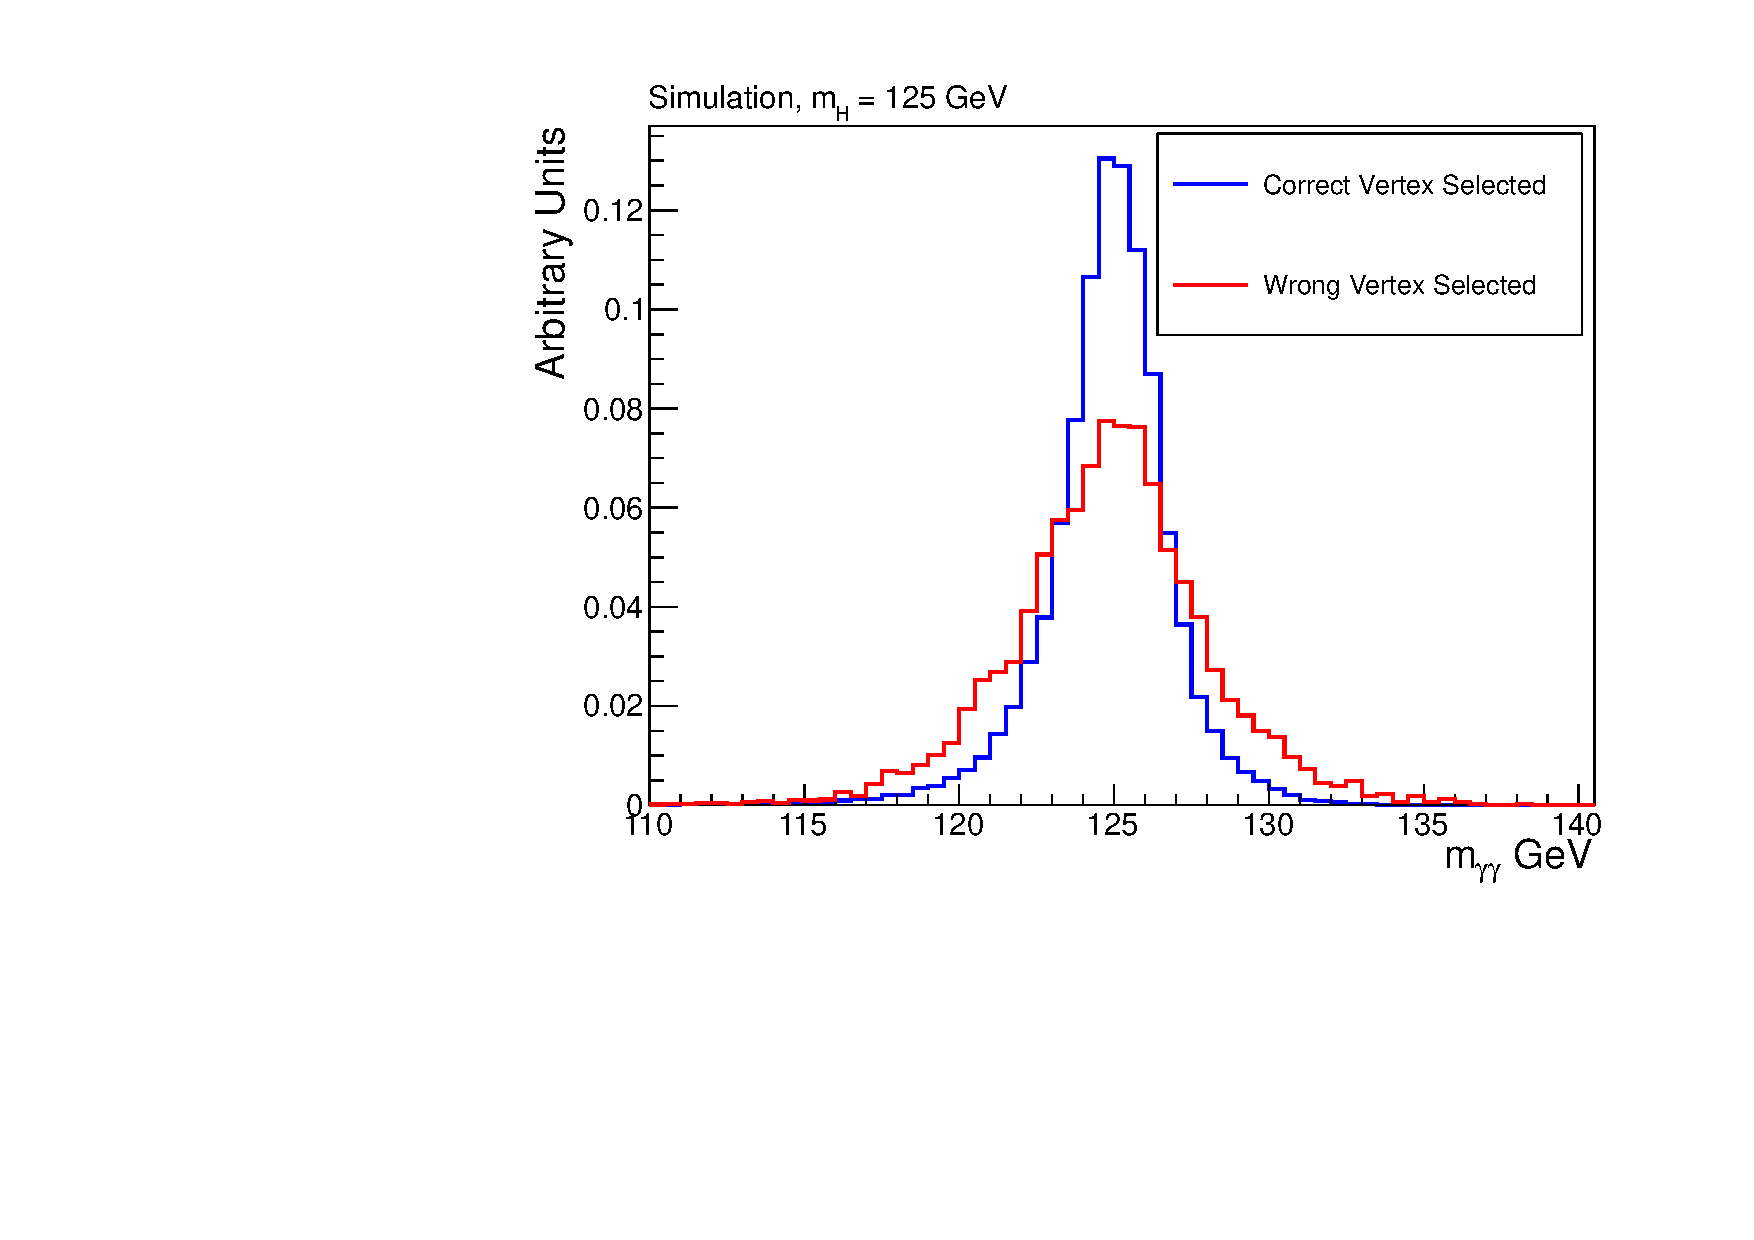
\includegraphics[width=.8\textwidth]{hgg7TeV/generalPlots/rightwrongvtxpeak.pdf}
\caption{Invariant mass peak in $\Hgg$ MC with $\mh=125$ GeV. The blue histogram is from events in which 
the generated vertex is within 10mm of the vertex assigned to the diphoton pair. The red histogram is 
from events in which the incorrect vertex is assigned. Both distributions are normalised to unit area for
ease of comparison.}
\label{fig:higgsrightwrongvertex}
\end{figure} 

A BDT was trained to rank the standard collection of reconstructed vertices.
The input variables are chosen to exploit the correlation between the diphoton system and the recoiling tracks.
These are the $\pt$-balance,
\begin{eqnarray}
	-\sum_{all tracks} \left(\ptvec^{track}\cdot \frac{\displaystyle \ptggvec}{\displaystyle \ptgg}\right), 
\end{eqnarray}
and the $\pt$-asymmetry calculated as,
\begin{eqnarray}
	\frac{\displaystyle |\sum_{all tracks} \ptvec^{track}| - \ptgg }{ \displaystyle|\sum_{all tracks} \ptvec^{track}|}.
\end{eqnarray}
In addition, the sum of the squares of the transverse momenta of all the tracks associated 
to a given vertex is included to preferentially select hard interactions. If at least one of the 
photons converts to an $e^{+}e^{-}$ pair, the difference between the position in $z$ as calculated 
using the electron-positron pair and that from the standard vertex, relative to the resolution in $z$, 
is included as an input variable. The BDT was trained on $\Hgg$ MC with a mass of 120 GeV. 
Figure~\ref{fig:vtxeffhmc} shows the fraction of events in a gluon-gluon MC sample in which 
the vertex with the highest BDT score is within 10mm of the true vertex as a function of $\pt^{H}$.
\begin{figure}
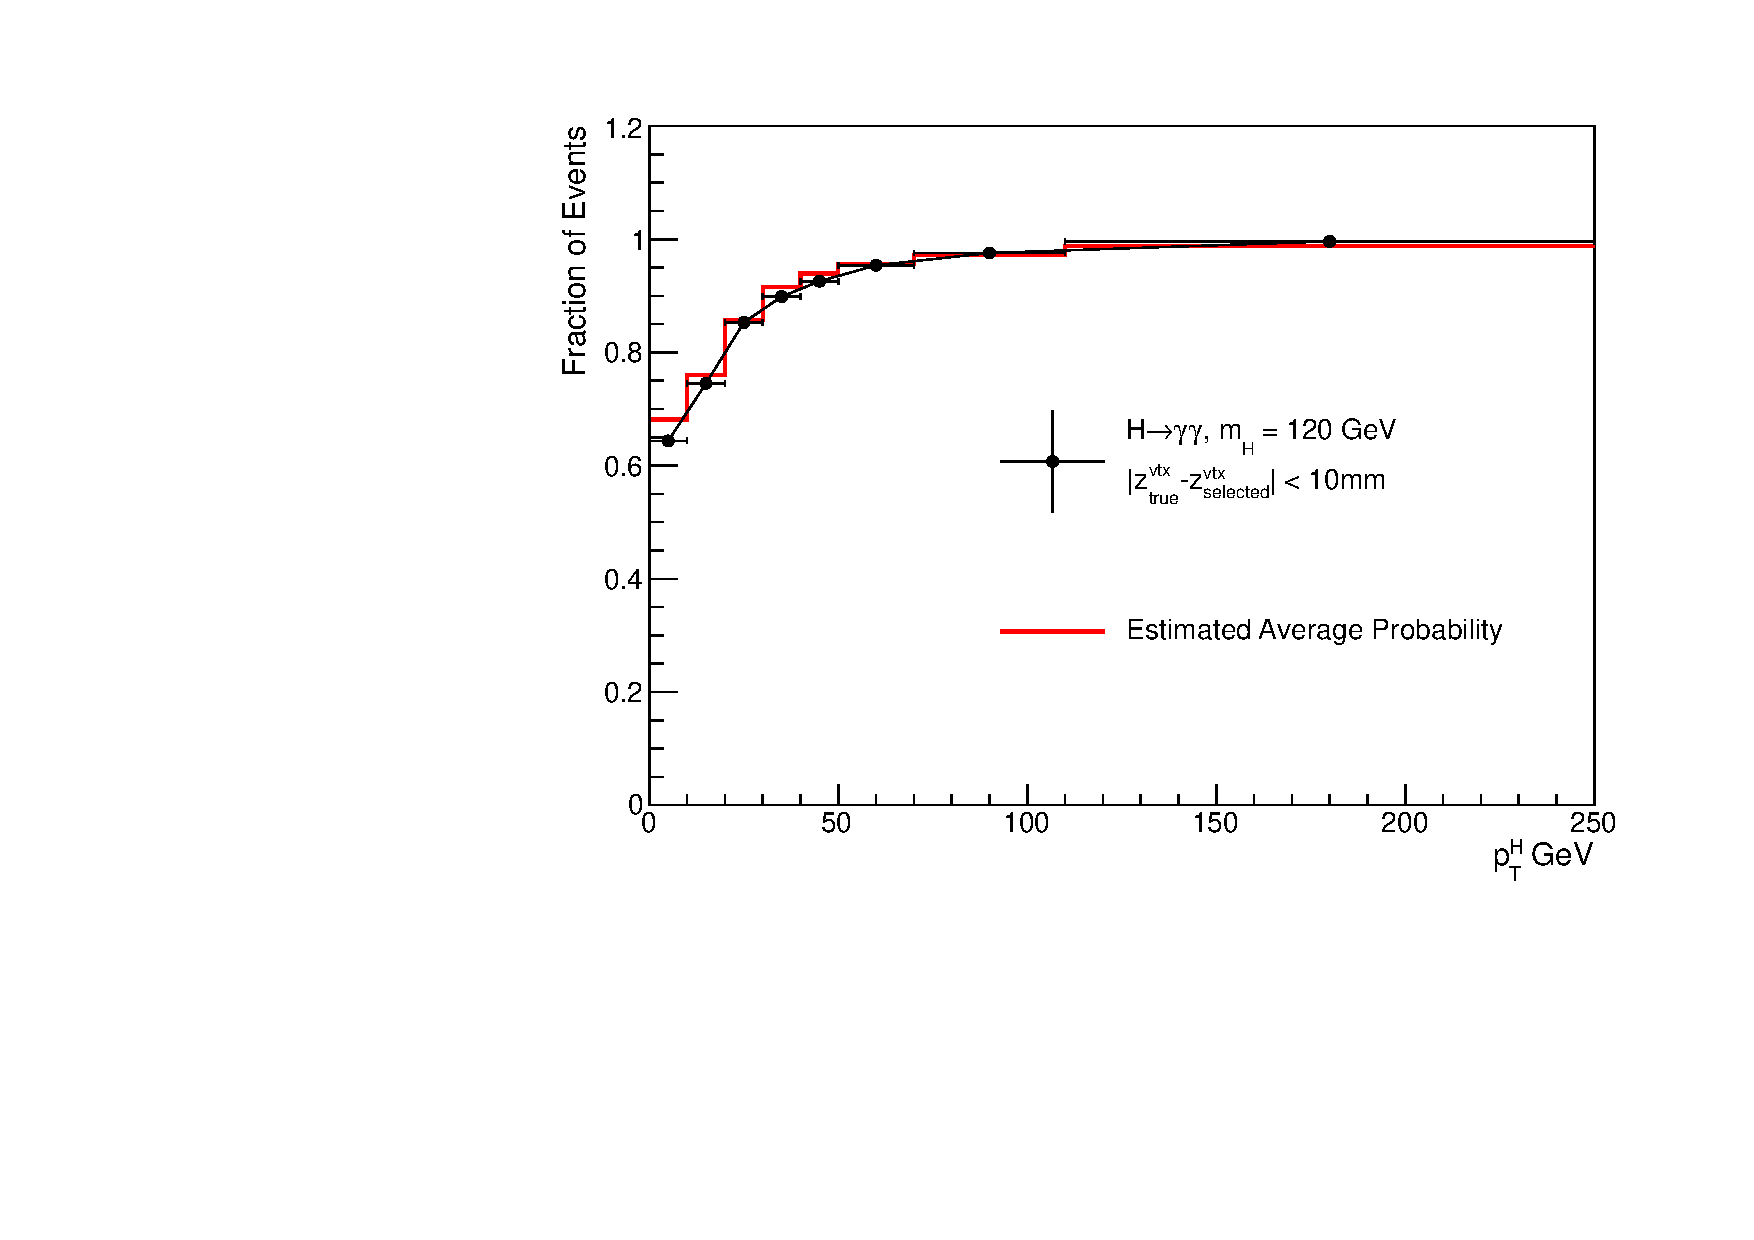
\includegraphics[width=.8\textwidth]{hgg7TeV/generalPlots/vtxEffHMC.pdf}
\caption{Fraction of simulated gluon-gluon fusion events in which the $z$ position of the selected vertex
is within 10mm of the true vertex as a function of Higgs boson $\pt$. The red histogram is the average 
probability to select the correct vertex in each bin estimated from the per-event BDT.}
\label{fig:vtxeffhmc}
\end{figure} 
The fraction of events in which this occurs in data is measured using $\Zmumu$ events
as a function of the $\pt$ of the $Z$ boson~\citep{AN-12-048}. 
Figure~\ref{fig:vtxzmumu} shows the fraction of events for which the chosen 
vertex is within 10mm of the 
true vertex as measured in $\Zmumu$ data and MC. 
The BDT (MVA) selection method described is compared with the standard CMS vertex ranking 
algorithm (RANK)~\citep{IN-11-014} which is less efficient for low $\pt^{Z}$.
The measurements in data are used to correct the Higgs signal MC for the purpose of signal modelling. 

\begin{figure}
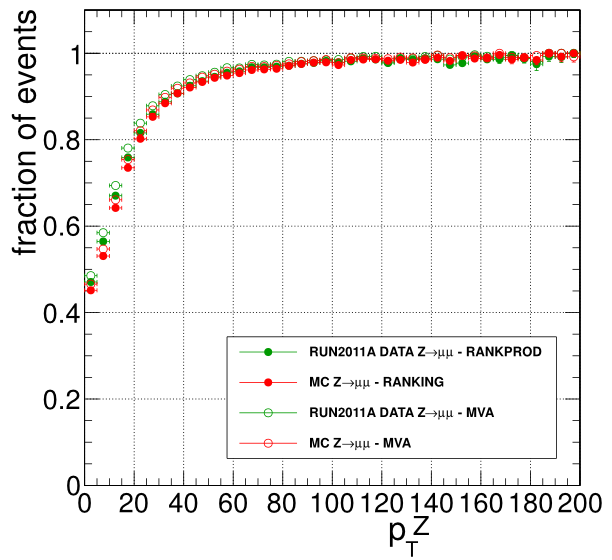
\includegraphics[width=.49\textwidth]{hgg7TeV/generalPlots/PT_vtx_z_2011A.png}
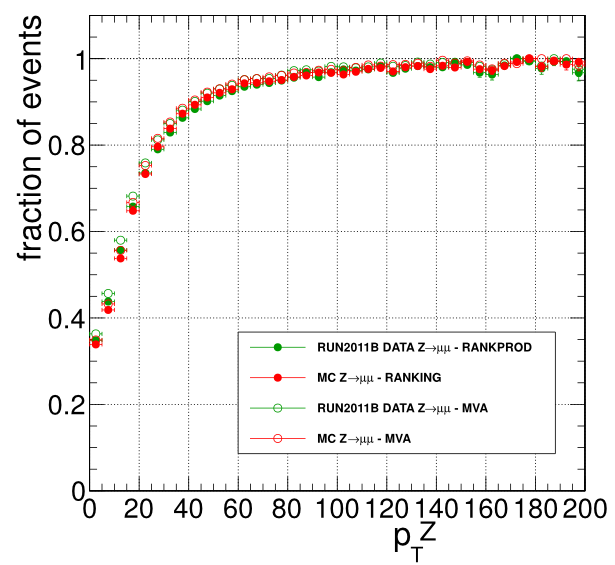
\includegraphics[width=.49\textwidth]{hgg7TeV/generalPlots/PT_vtx_z_2011B.png}
\caption{Fraction of $\Zmumu$ events in which the selected vertex is with 10mm of the 
true vertex in Run 2011A (left) and Run 2011B (right) data and MC as a function of $\pt^{Z}$~\citep{AN-12-048}. 
The BDT selection, labelled MVA, is shown by the open circles where the ranking method, labelled RANK 
is shown as points.}
\label{fig:vtxzmumu}
\end{figure} 

A second, per-event, BDT is trained using the output of the first to identify 
under which conditions the correct vertex is selected. The output of this BDT is then used to 
calculate the probability in a given event that the correct vertex is assigned. The red line in Figure~\ref{fig:vtxeffhmc}
shows a comparison of the per-event vertex probability estimated from the second BDT against the 
fraction of the events in which the selected vertex is located within 10mm from the true vertex. The per-event vertex probability 
estimate provides a good model of the actual fraction of events in which the correct vertex is selected.

\subsection{Photon Identification}
\label{sec:photonidentification}

A large portion of the fake background in the $\Hgg$ search is due to high momentum neutral mesons
which decay to two photons where both the photons are combined into the same supercluster~\citep{HIG-11-033}. 
Information from the shower shape of the photon supercluster can be used, in addition to the 
energy isolation within the calorimeter, in order to distinguish these from prompt photons
from the primary interaction point. A BDT was trained on MC events to combine the relevant information
into a single photon identification (ID) discriminator. The signal used for the training was taken from 
simulated $\Hgg$ events with a Higgs boson mass of 121 GeV while the background was 
taken from non-prompt photons in the gamma+jet (prompt-fake) sample.
Before training, events are required to pass a loose pre-selection designed to avoid training 
where the MC is unable to properly describe the data and to match the variables used in the trigger~\citep{AN-12-048}.
In addition, photon candidates are removed if there is a reconstructed electron matched to the 
photon supercluster with no matching conversion reconstruction. This greatly reduces the contribution
from electrons in $\Zee$ faking photons. The same pre-selection is applied to all MC and data for extracting the signal.
The efficiency of the pre-selection for signal was measured in $\Zee$ data and MC using a tag-and-probe 
method~\citep{AN-12-116}. 

The measurement is made using events which are selected using a dielectron
trigger with supercluster transverse energies of at least 20 GeV. The two objects are then 
randomly assigned as either the ``tag'' or ``probe'' candidate. The tags are then required to 
pass a tight electron selection based on their isolation and supercluster shower shape.
Events are then split into those in which the probe candidate passes or fails the pre-selection
and the ratio of signal events, after background subtraction, in each class provides the 
efficiency measurement of the pre-selection. For the pre-selection efficiency measurement, 
the background subtraction is performed using a likelihood fit to the invariant 
mass of the tag-probe pair, modelling the signal with a Breit-Wigner convoluted with a 
Crystal Ball and the background with an exponential function. 
Both models are multiplied by an error function of the form,
\begin{equation}
\mathrm{erf}(x)\propto \int_{0}^{\frac{x-\mu}{\sigma}} e^{-t^{2}}dt,
\end{equation}
with parameters $\mu$ and $\sigma$ freely floating. The measurement is performed
in four probe categories depending on the $\rnine$ and $|\eta|$ of its supercluster.
The results are shown in Table~\ref{tab:sigeffpresel}. 

\begin{table}
\begin{tabular}{| l | c | c | c |}
\hline
\textbf{Category} & \textbf{Data} & \textbf{MC} & \textbf{Data/MC} \\
\hline
EB $\rnine>0.9$ & 0.927 $\pm$ 0.001 & 0.928 $\pm$ 0.001 &0.999 $\pm$ 0.001 \\
EB $\rnine<0.9$ & 0.888 $\pm$ 0.002 & 0.903 $\pm$ 0.001 &0.984 $\pm$ 0.003 \\
EE $\rnine>0.9$ & 0.944 $\pm$ 0.001 & 0.938 $\pm$ 0.001 &1.006 $\pm$ 0.001 \\
EE $\rnine<0.9$ & 0.864 $\pm$ 0.001 & 0.852 $\pm$ 0.001 &1.014 $\pm$ 0.001 \\
\hline
\end{tabular}
\caption{Signal efficiency for the preselection measured in data and MC using tag-and-probe in
$\Zee$ events. The Data/MC ratios are applied as corrections to the signal MC for the purposes
of signal modelling. The uncertainties listed here are statistical only.}
\label{tab:sigeffpresel}
\end{table}

The input variables are chosen to be insensitive to the kinematics of the diphoton system itself
including the diphoton invariant mass. The first set of variables describe the shower shape of the 
supercluster: $\hoe$ (the ratio of energy deposited in the HCAL behind the ECAL to that of the supercluster), 
$\sigieie$, $\rnine$ and the energy weighted widths of the supercluster in
$\eta$ and $\phi$ ($\sigma_{\eta},~\sigma_{\phi}$). The $\eta$ of the supercluster is 
included as the shower shape is dependent on the position within the calorimeter. 
The second set of input variables describe the
isolation of the photon in the calorimeter and tracker scaled to account for 
the additional expected energy density due to pileup, $\rho$~\citep{2011JInst611002C}. 
These are: the sum of the track isolation, 
calculated relative to the chosen vertex and the vertex giving the maximum track isolation,
ECAL and HCAL isolations in cones with $\Delta R<0.3$ minus $\rho$ times the effective area 
of the cone~\citep{2011JInst611002C}; 
and the absolute ECAL and HCAL isolations within cones of $\Delta R <0.3$ and $\Delta R<0.4$ 
respectively. In addition, the number of reconstructed vertices in the bunch crossing is included
to reduce the pileup dependence of the isolation variables. 

Separate BDTs are trained for the ECAL barrel and endcaps as the shower
shape and isolation variables are rather distinct between the two. 
A cut is made on the photon ID BDT output to select events used for the signal extraction which
keeps practically all ($>99\%$) of the signal while removing around 22\% of background events.
The cut is chosen to be loose as the output of the photon ID will be used as an input to the 
event selection (diphoton BDT) as described in Section~\ref{sec:diphotonbdt}. 

\section{Event Selection}
\label{sec:eventselection}

In addition to passing the pre-selection, the two photons are required to pass mass-dependent transverse 
momenta cuts, $p_{T}/\mgg > 1/3, ~1/4$ for the leading and sub-leading photon respectively.
Where more than one diphoton pair in an event satisfies these criteria, the pair which has the largest
sum of photon transverse momenta is selected as the Higgs boson candidate.
The final selection of diphoton candidates used for the signal extraction is based on using as much information 
in the event as possible to distinguish likely signal candidate events from the background. Although the 
photon ID BDT is successful at rejecting fake backgrounds, a large portion of the background is due to
real prompt diphotons from QCD processes. In order to distinguish these from a Higgs signal, 
the specific kinematics and topology of the event are exploited.

\subsection{Diphoton BDT}
\label{sec:diphotonbdt}
A BDT was trained to utilise the kinematics of the selected diphoton pair to discriminate prompt photons
from QCD background from those produced by the decay $\Hgg$. The BDT was trained using the prompt-prompt, prompt-fake
and fake-fake samples for background and Higgs MC with a mass of 123 GeV for signal.
As the mass of the Higgs boson is unknown, the search is performed under different mass hypotheses.
In order to allow for the application of the same selection to the data under any mass hypothesis,
the input variables to the BDT are chosen to be mass-independent. In addition, this allows
for a fully data-driven estimation of the background shape as described in Section~\ref{sec:backgroundmodel}.
The input variables which describe the kinematics are:
the relative transverse momenta of the leading and sub-leading photons ($\pt^{1}/\mgg,~\pt^{2}/\mgg$ respectively), 
their pseudo-rapidities, $\eta^{1},~\eta^{2}$ and the cosine of the 
angle between the two photons in the transverse plane $cos(\Delta\phi)=cos(\phi^{1}-\phi^{2})$.
In addition, information regarding the quality
of the objects, the two photons and the selected vertex, is included in the form of the output of the 
photon ID and the vertex probability BDTs. The per-photon resolution estimate, $\sigma_{E}$ is combined for
each photon to produce a per-event mass resolution estimate under the assumption that 
the correct vertex is selected, $\sigma_{\mgg}(\mathrm{right-vertex})$,
\begin{equation}
\sigma_{\mgg} (\mathrm{right-vtx}) = \frac{\displaystyle \mgg}{\displaystyle 2} 
\sqrt{ \left( \frac{\displaystyle {\sigma_{E}^{1}}}{\displaystyle E^{1} } \right)^{2}
     + \left( \frac{\displaystyle {\sigma_{E}^{2}}}{\displaystyle E^{2} } \right)^{2}
     }
\end{equation}
where $E^{1}$ and $E^{2}$ are the energies of the two photons.

Since the correct vertex is not always selected, the mass resolution assuming the incorrect vertex is chosen
is calculated using the average length of the region in which the two proton beams collide in data, $\sigma_{Z}=5.8$cm. In this case, the distance 
between the selected and true vertex will be distributed as a Gaussian with width $\sqrt{2}\sigma_{Z}$.
The contribution to the resolution, $\sigma_{\mgg}^{vtx}$, can be calculated analytically given the positions of
the two photons. The mass resolution estimator under the assumption that the incorrect vertex is chosen is 
given by the sum in quadrature of $\sigma_{\mgg}^{vtx}$ with the mass resolution assuming the correct vertex is chosen.
Both estimators for the mass resolution relative to the invariant mass, $\sigma_{\mgg}/\mgg~$ right/wrong-vtx, 
are included as inputs to the diphoton BDT.  
Figures~\ref{fig:diphotonbdtvars1} and~\ref{fig:diphotonbdtvars2} show the input variables from the 
final set of selected diphoton candidates in data and MC. 
The expectation in each plot from a SM Higgs boson with a mass of 125 GeV, scaled by 10, is shown in red. 
The invariant mass distribution in data and MC for events passing the full
selection is given in Figure~\ref{fig:massmcdata}. After the application of the full selection, 
the total background contains around 76\% prompt diphoton events.
Figure~\ref{fig:diphotonBDT} shows the diphoton BDT distribution in data and MC.
The final events used for the signal extraction are selected as those with a diphoton BDT output greater than 0.05. 
This cut was chosen following an optimization study to minimize the expected exclusion limit in the absence of signal.
Events below this cut value were found to provide negligible improvement in the expected limit~\citep{AN-12-048}.

\begin{figure}[hbt!]
  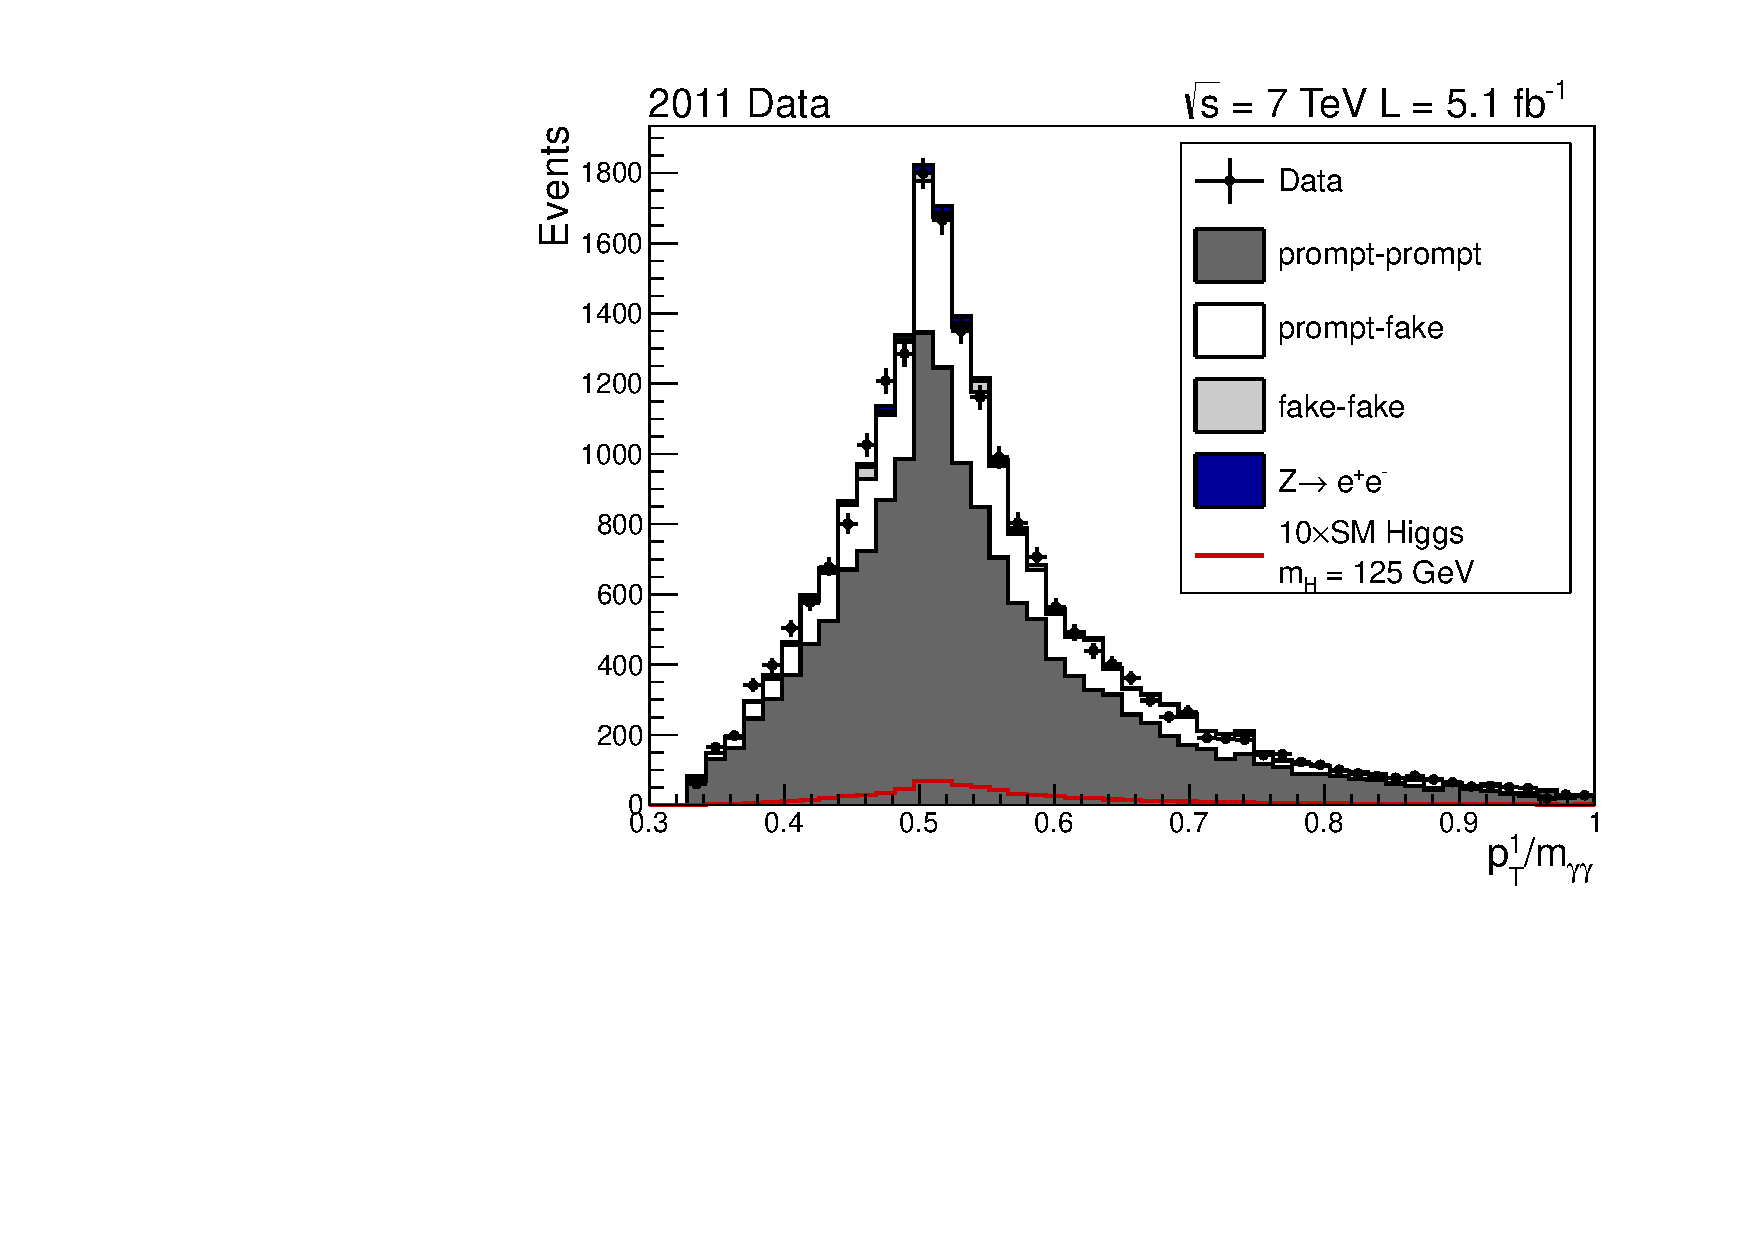
\includegraphics[width=0.48\textwidth]{hgg7TeV/variablePlots/pt_1om}
  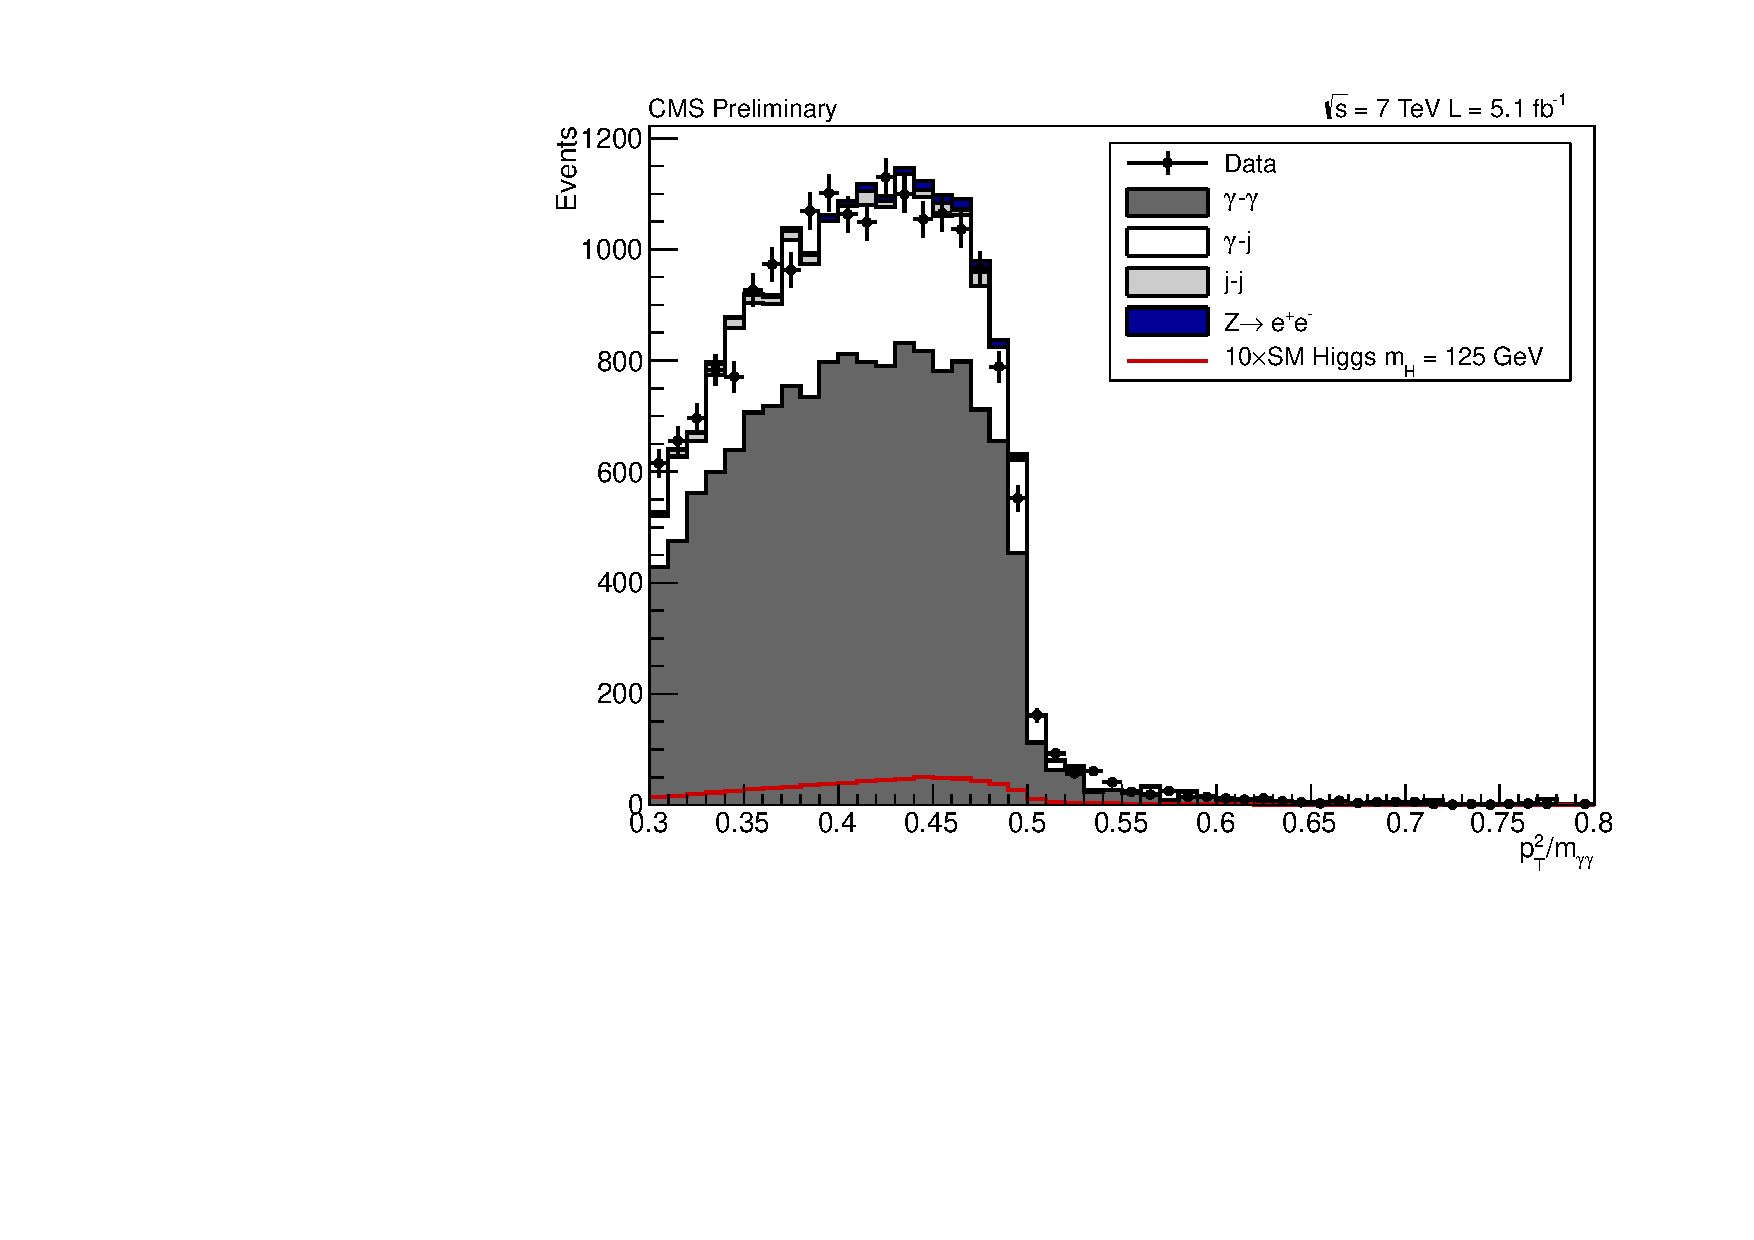
\includegraphics[width=0.48\textwidth]{hgg7TeV/variablePlots/pt_2om}\\
  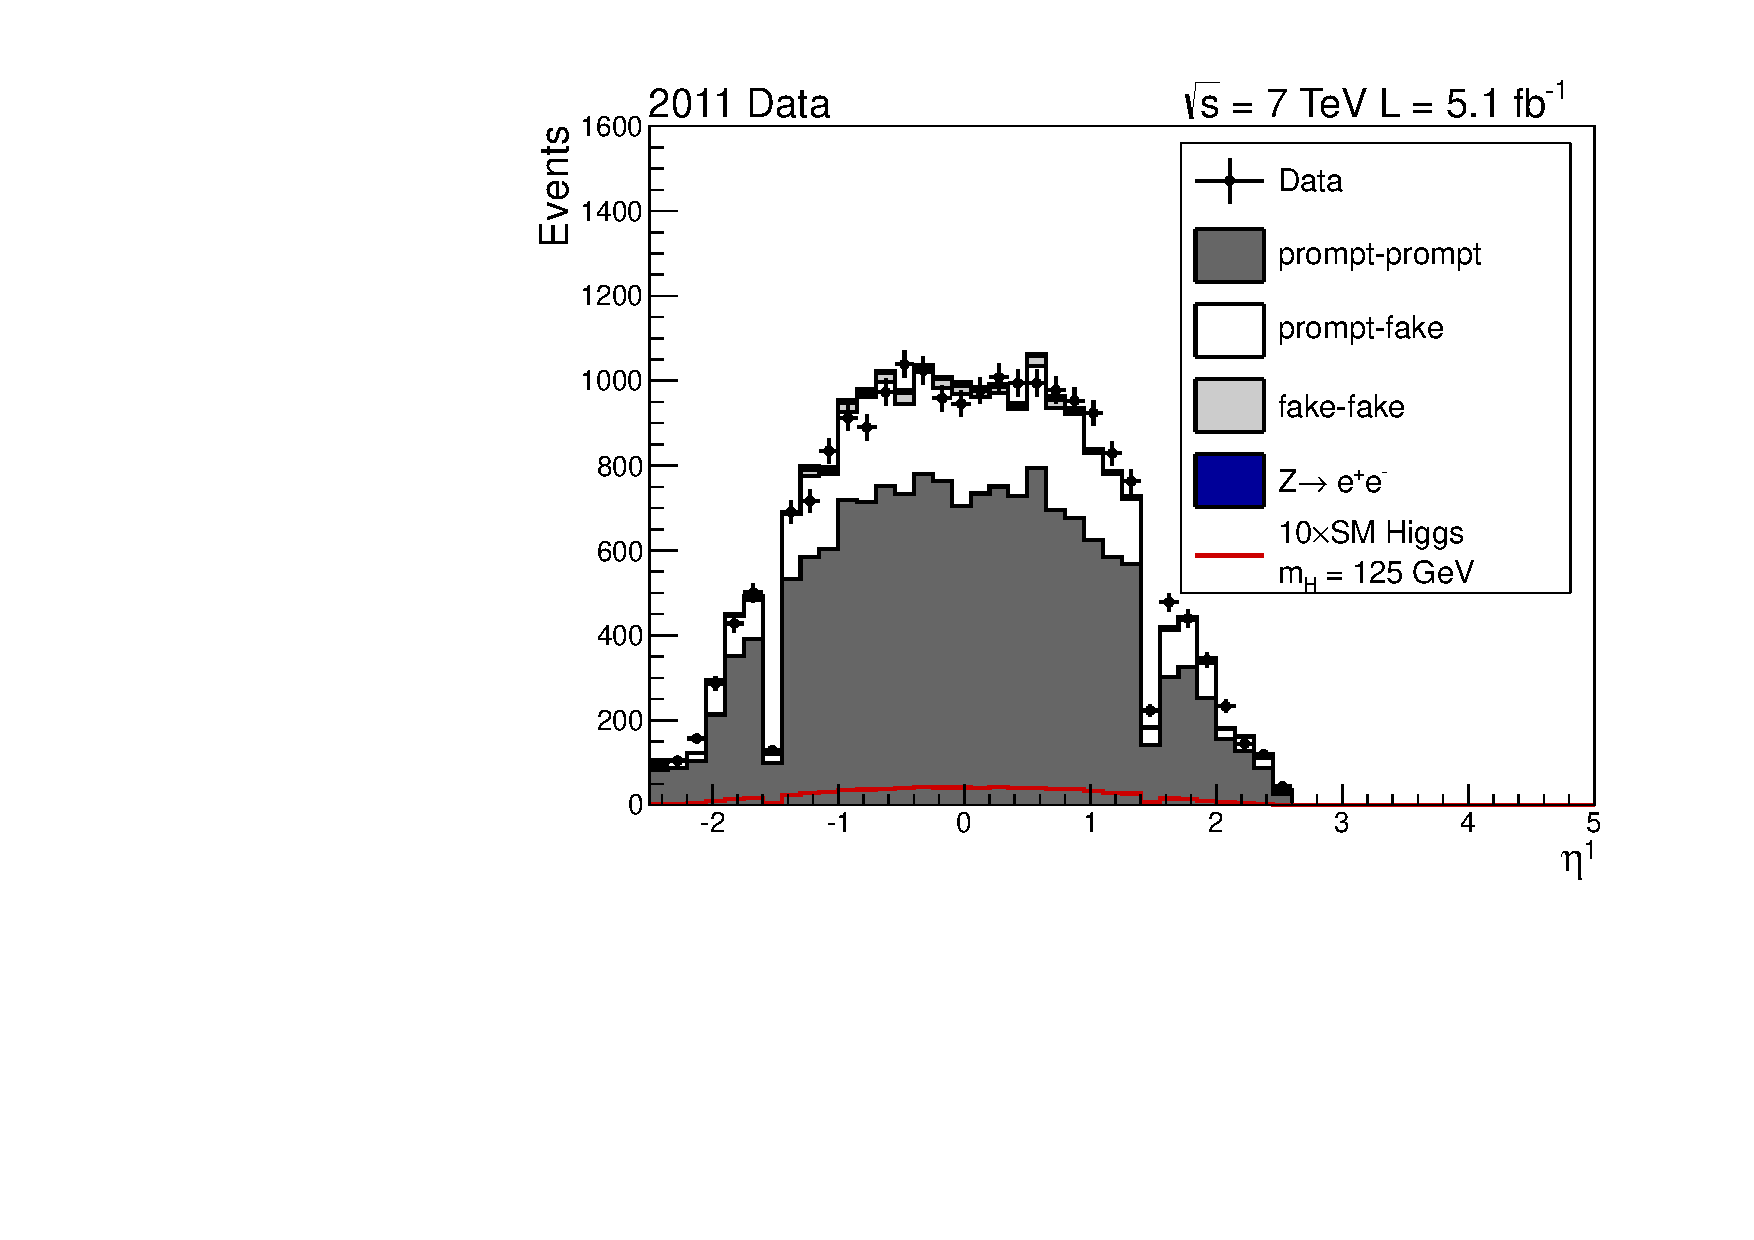
\includegraphics[width=0.48\textwidth]{hgg7TeV/variablePlots/phoeta_1}
  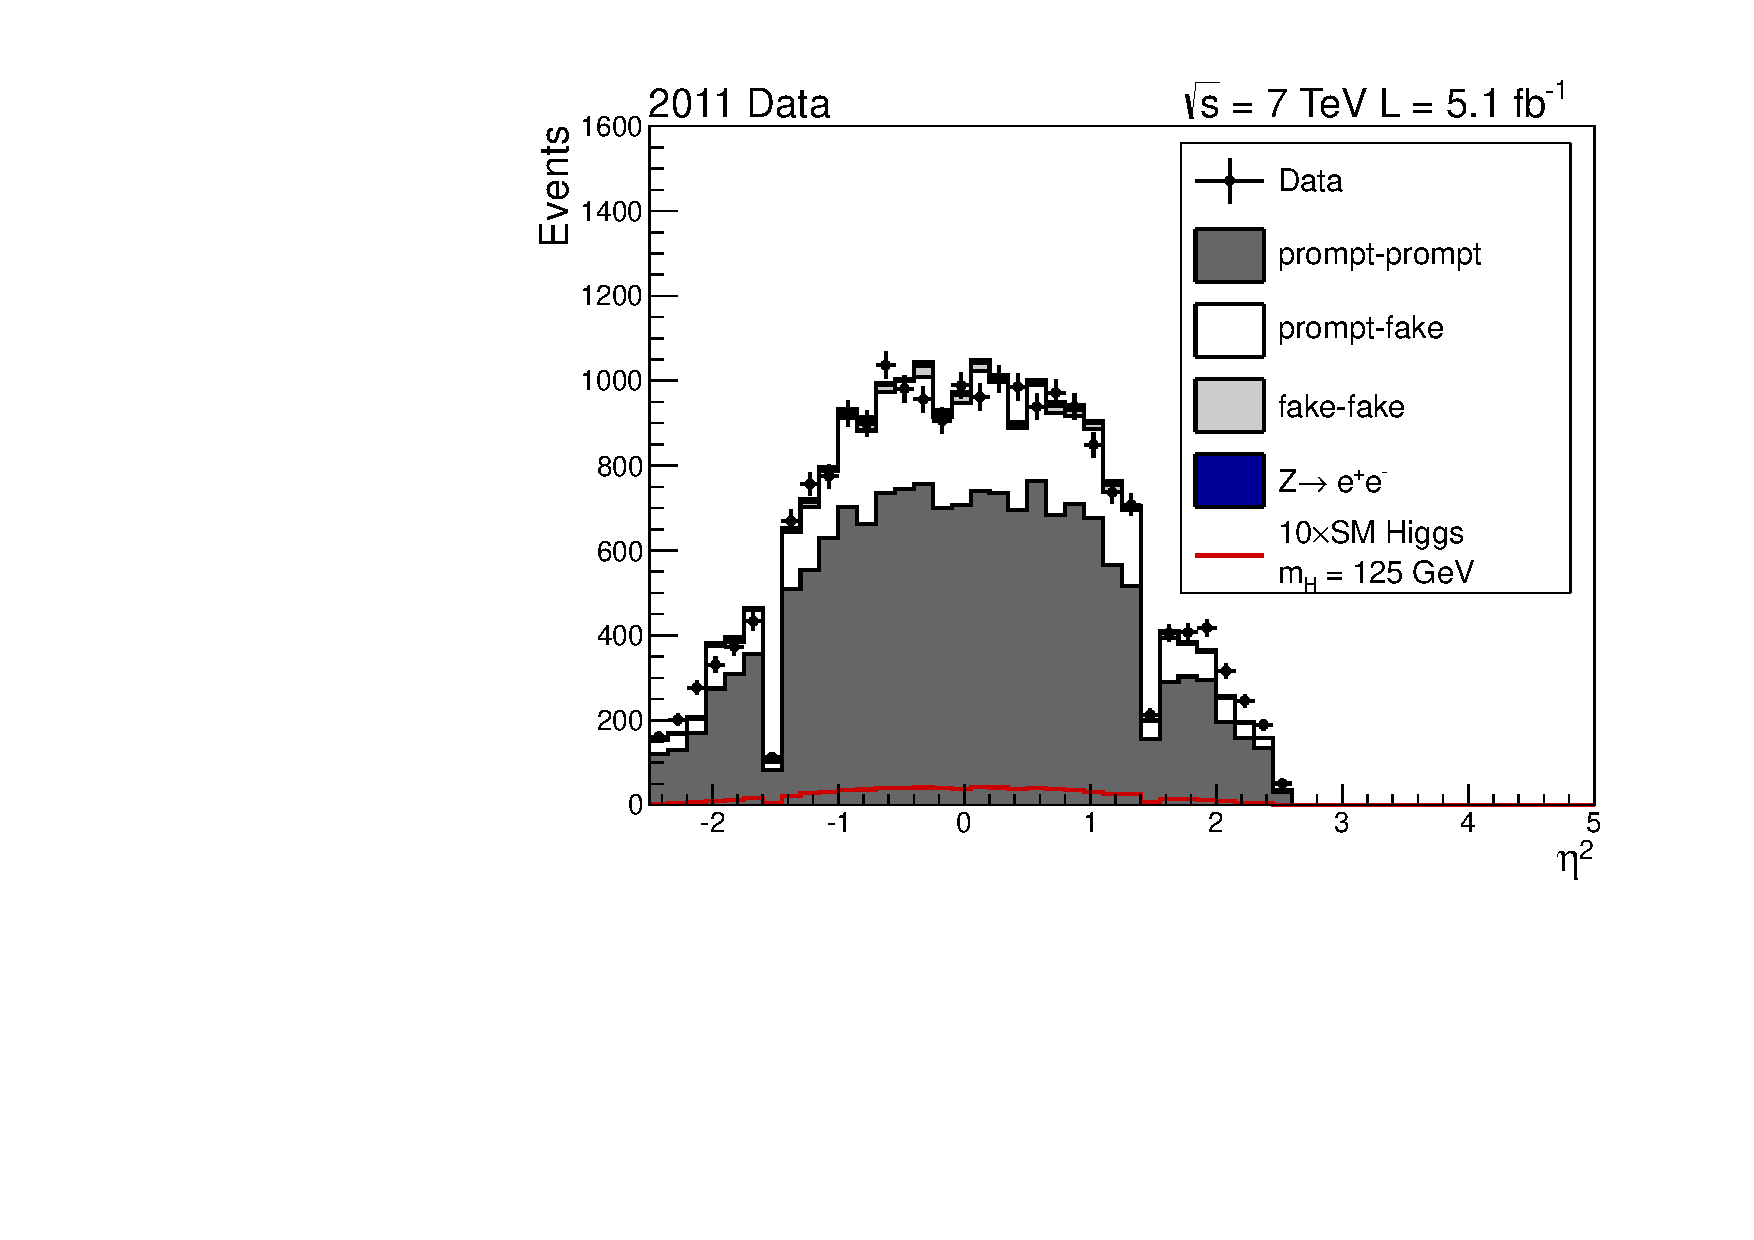
\includegraphics[width=0.48\textwidth]{hgg7TeV/variablePlots/phoeta_2}\\
  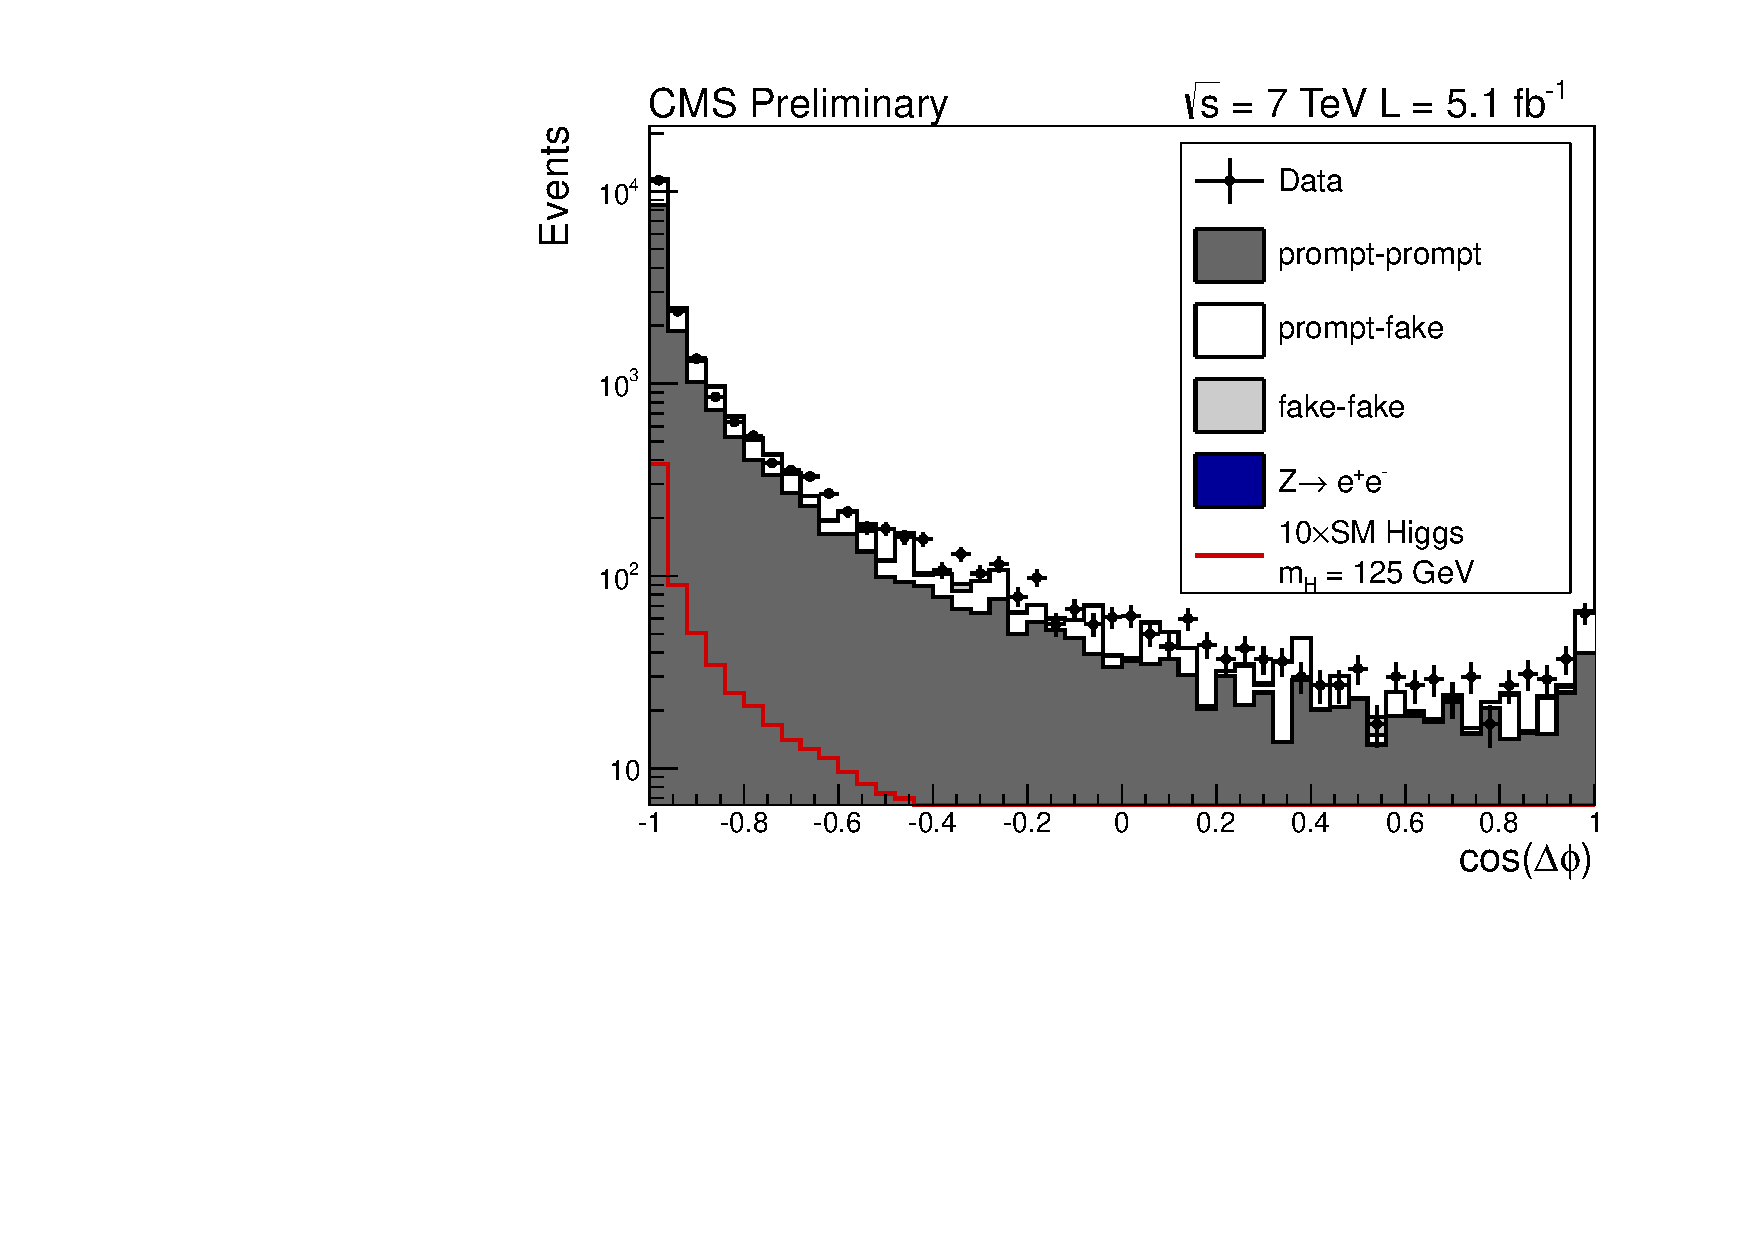
\includegraphics[width=0.48\textwidth]{hgg7TeV/variablePlots/cosdphi}
 \caption{Kinematic inputs to the diphoton BDT in data and MC. 
	  The distributions are for events which pass the full selection 
	  including a cut on the diphoton BDT output of 0.05.
 	  The expectation from a SM Higgs boson with 125 GeV is shown in red.}
 \label{fig:diphotonbdtvars1}
\end{figure}

\begin{figure}[hbt!]
  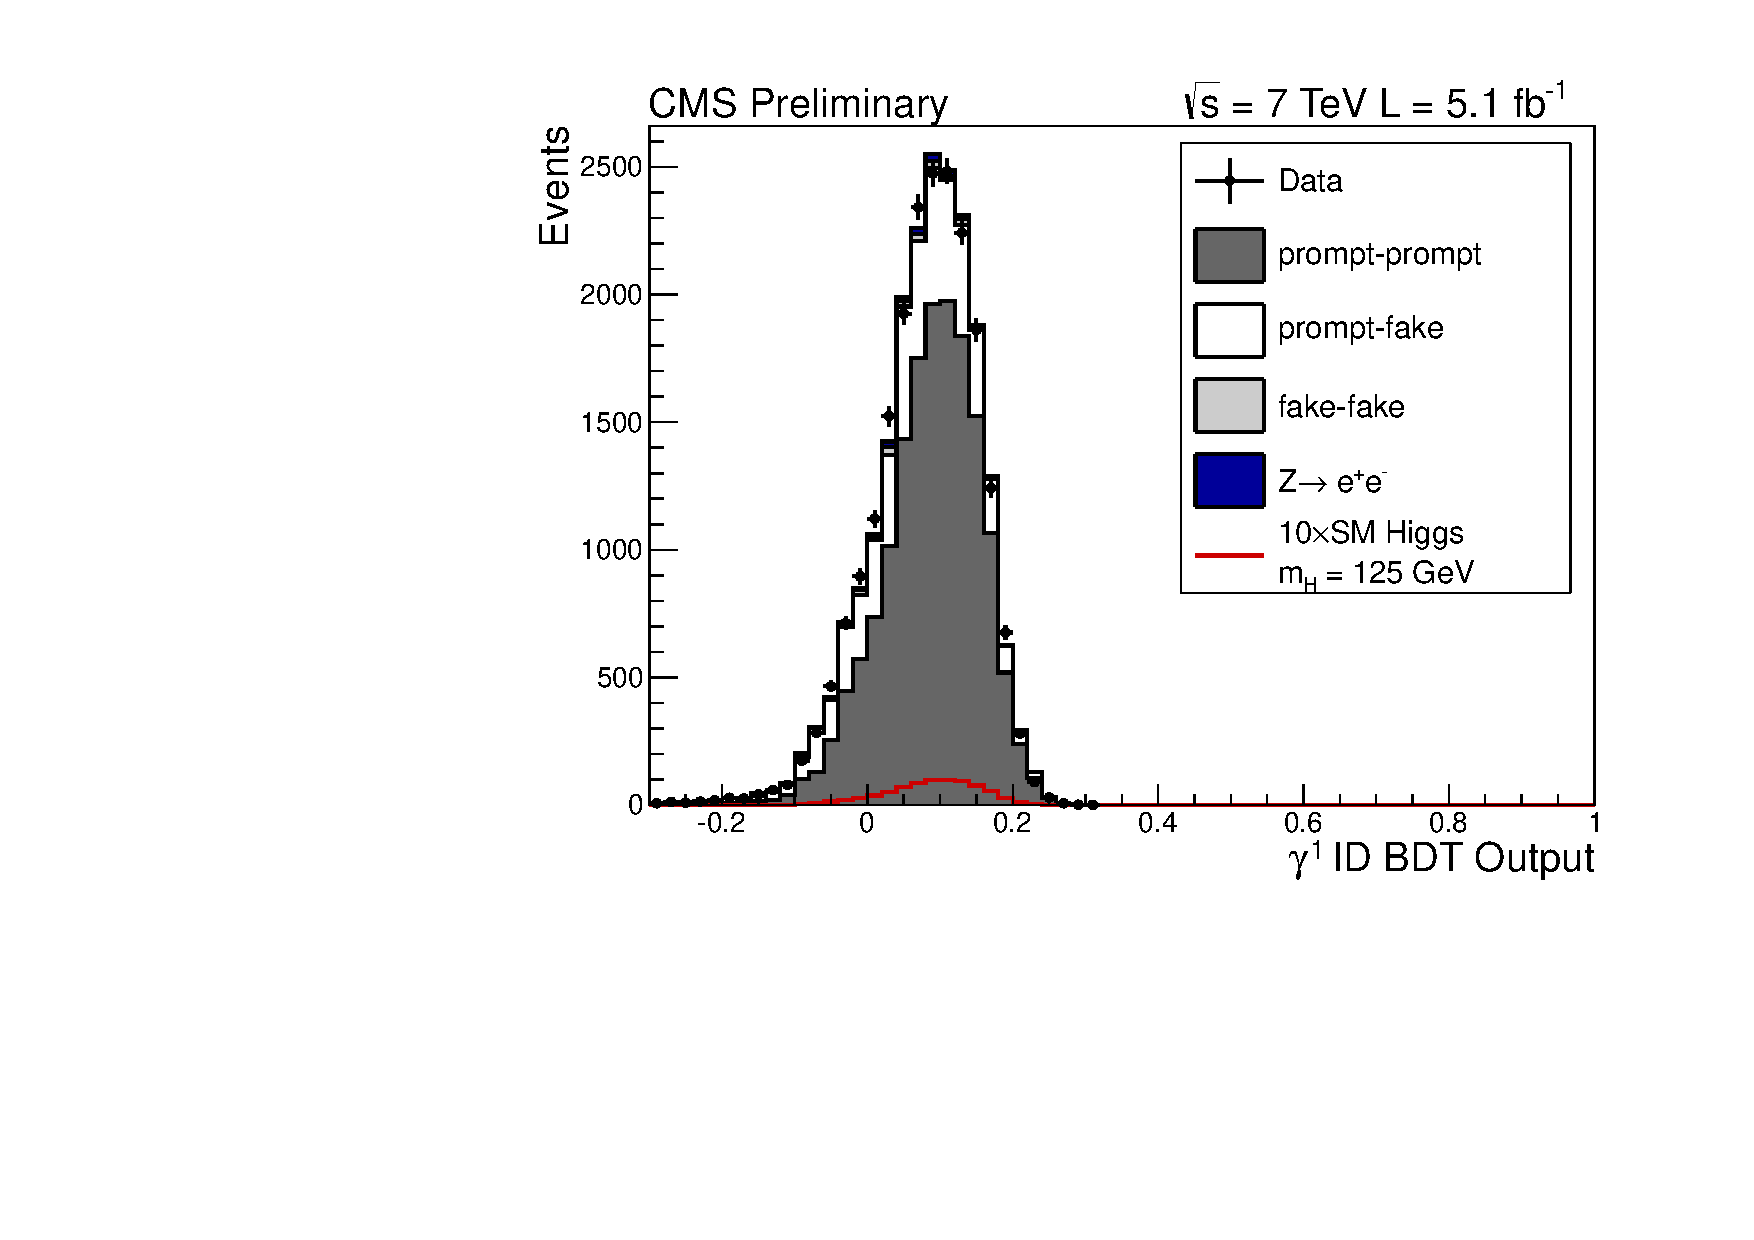
\includegraphics[width=0.48\textwidth]{hgg7TeV/variablePlots/phoid_1}
  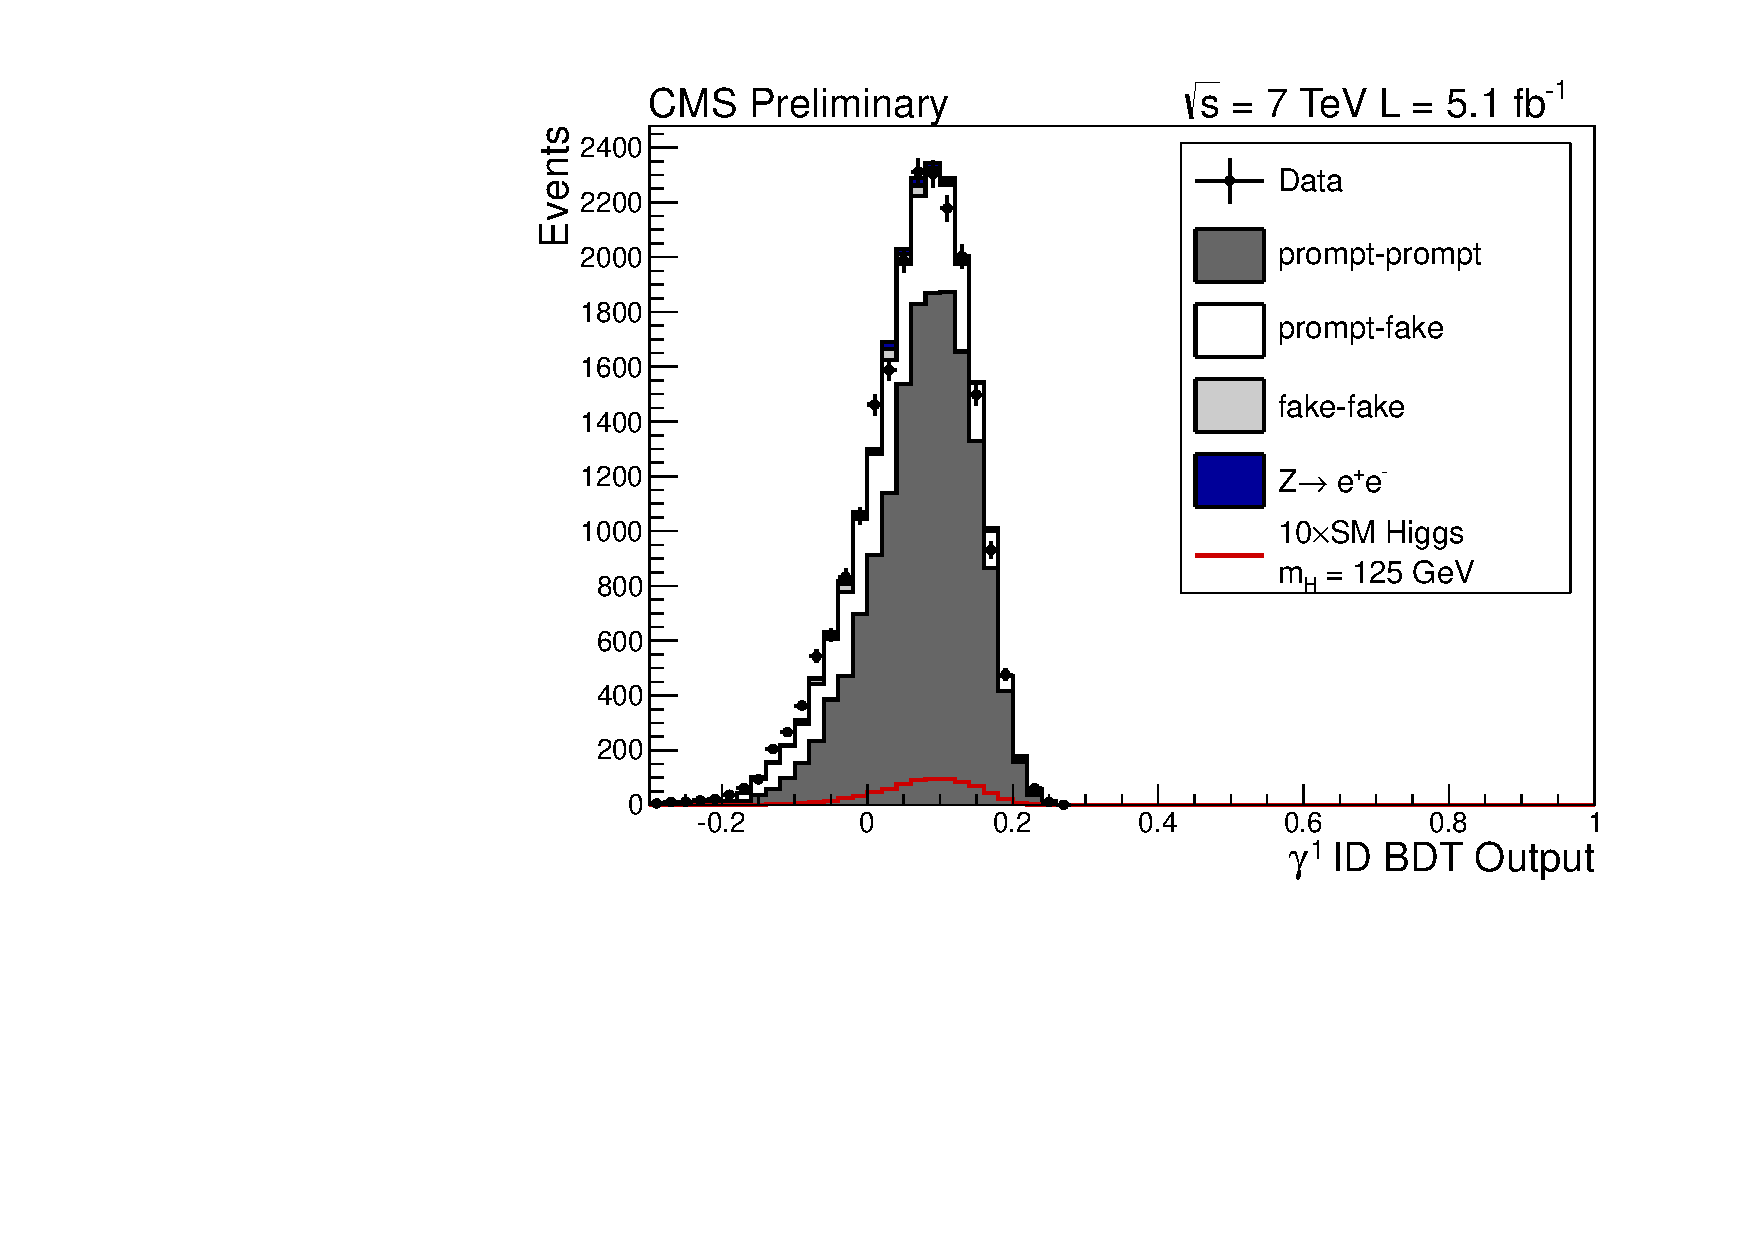
\includegraphics[width=0.48\textwidth]{hgg7TeV/variablePlots/phoid_2}\\
  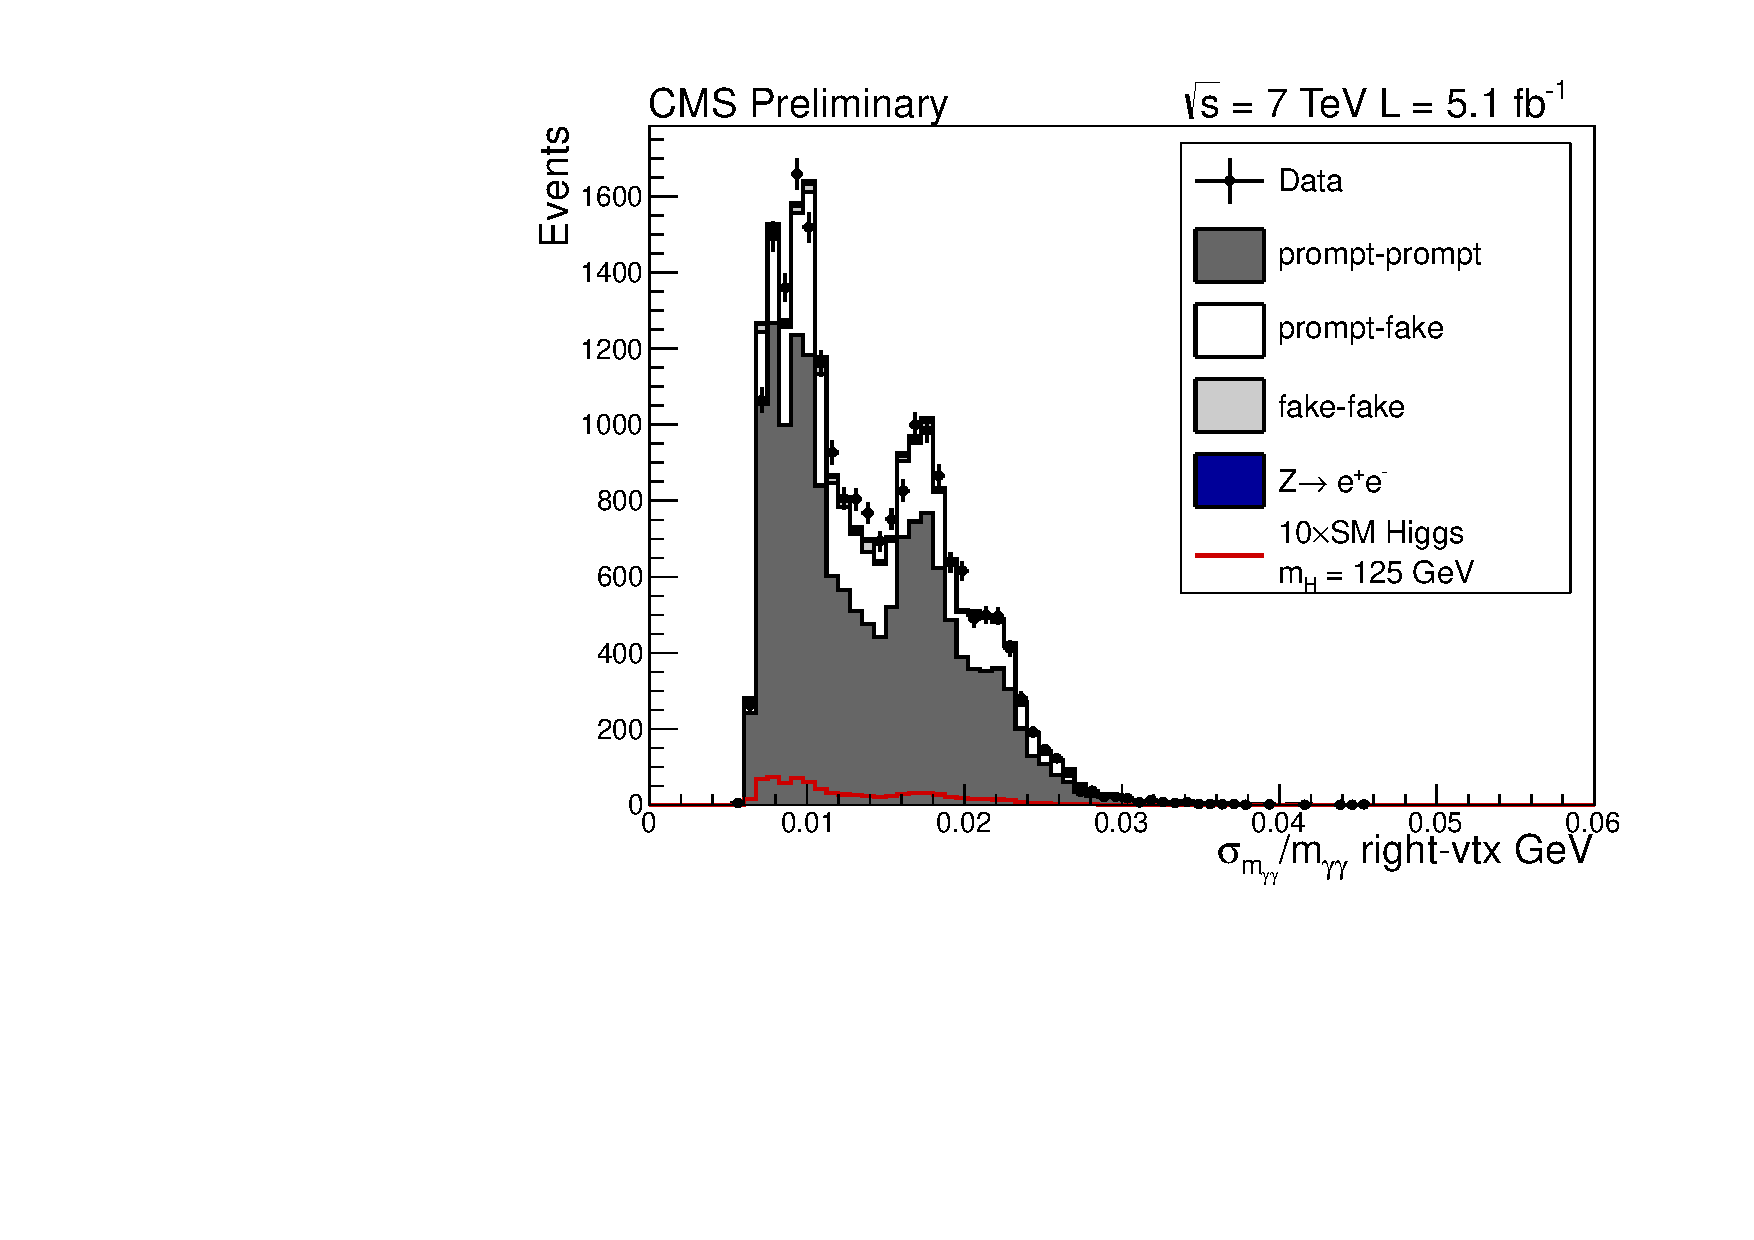
\includegraphics[width=0.48\textwidth]{hgg7TeV/variablePlots/sigmrv}
  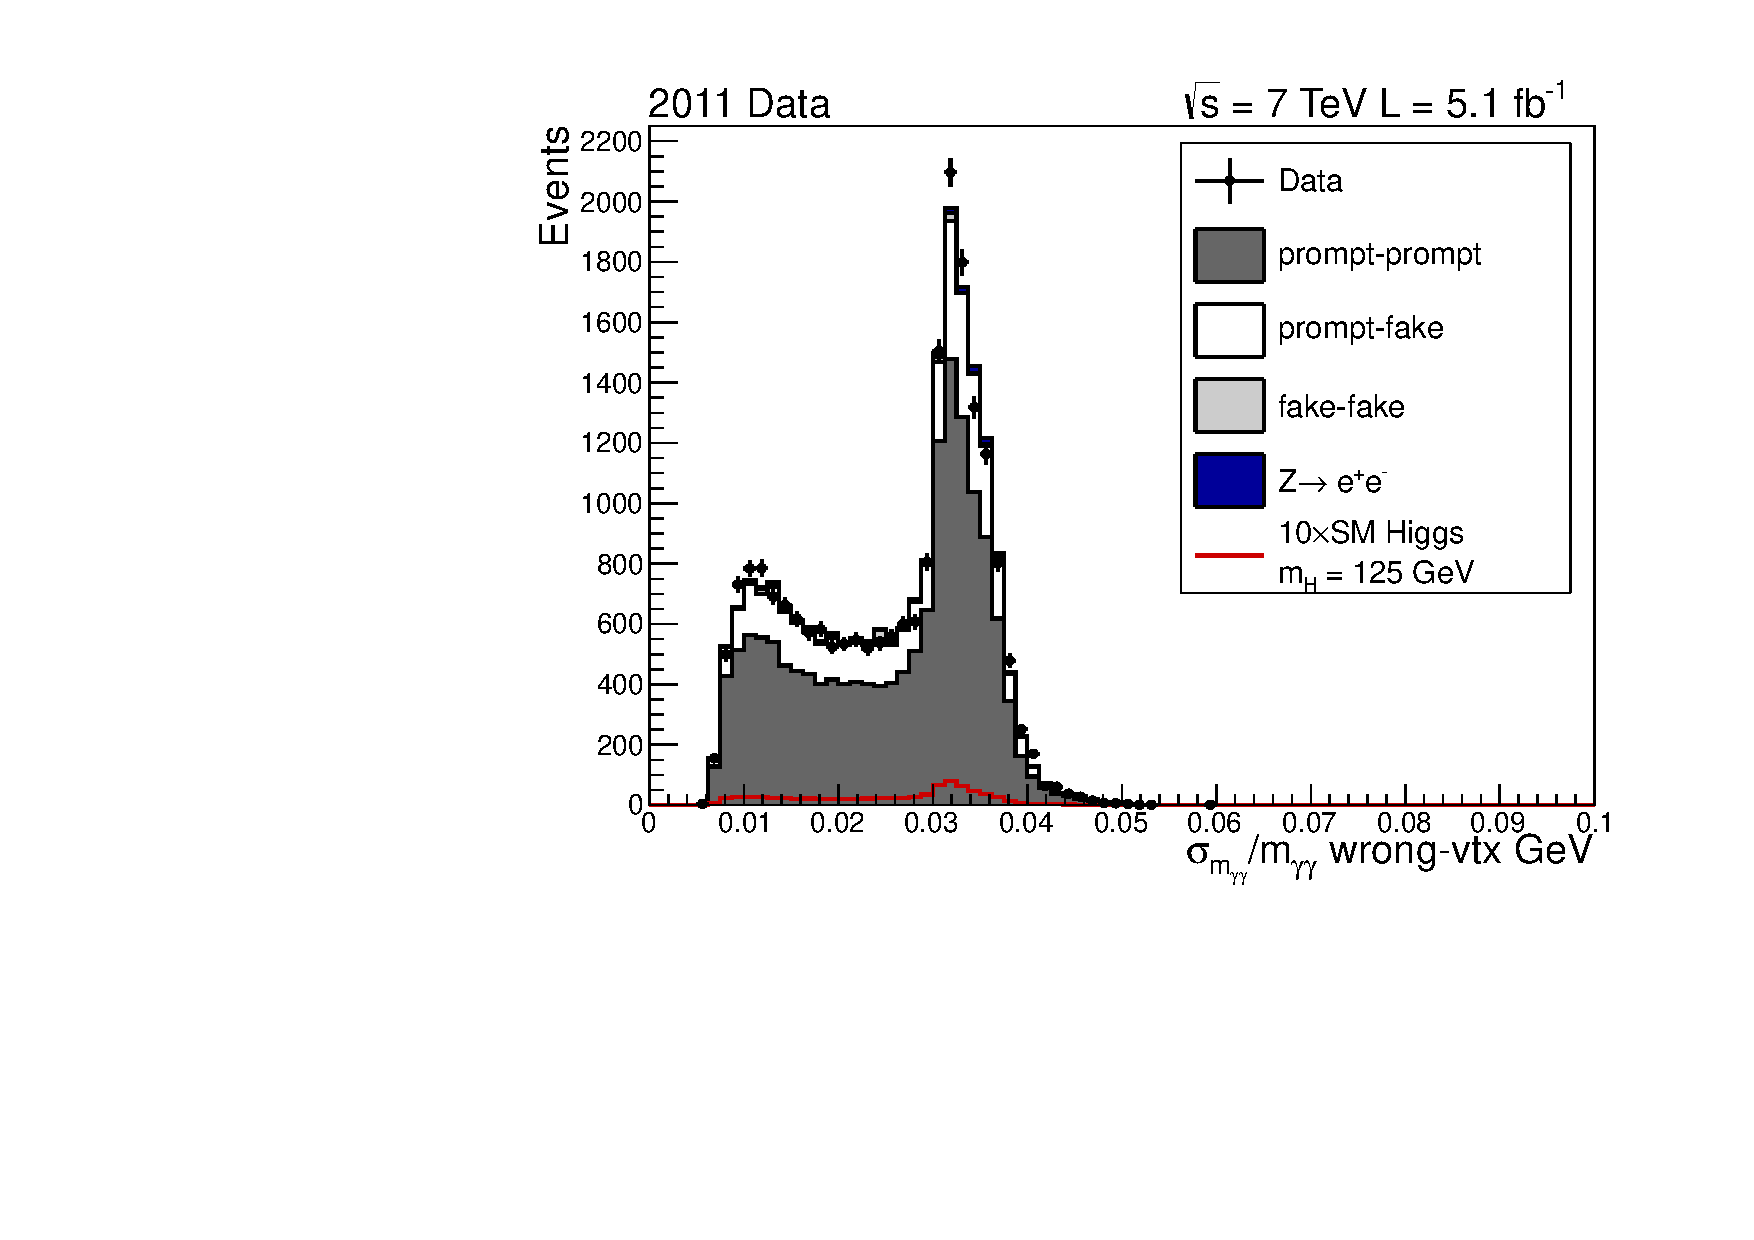
\includegraphics[width=0.48\textwidth]{hgg7TeV/variablePlots/sigmwv}
 \caption{Additional input variables to the diphoton BDT in data and MC. 
	  The distributions are for events which pass the full selection 
	  including a cut on the diphoton BDT output of 0.05.
 	  The expectation from a SM Higgs boson with 125 GeV is shown in red.}
 \label{fig:diphotonbdtvars2}
\end{figure}

\begin{figure}[hbt!]
 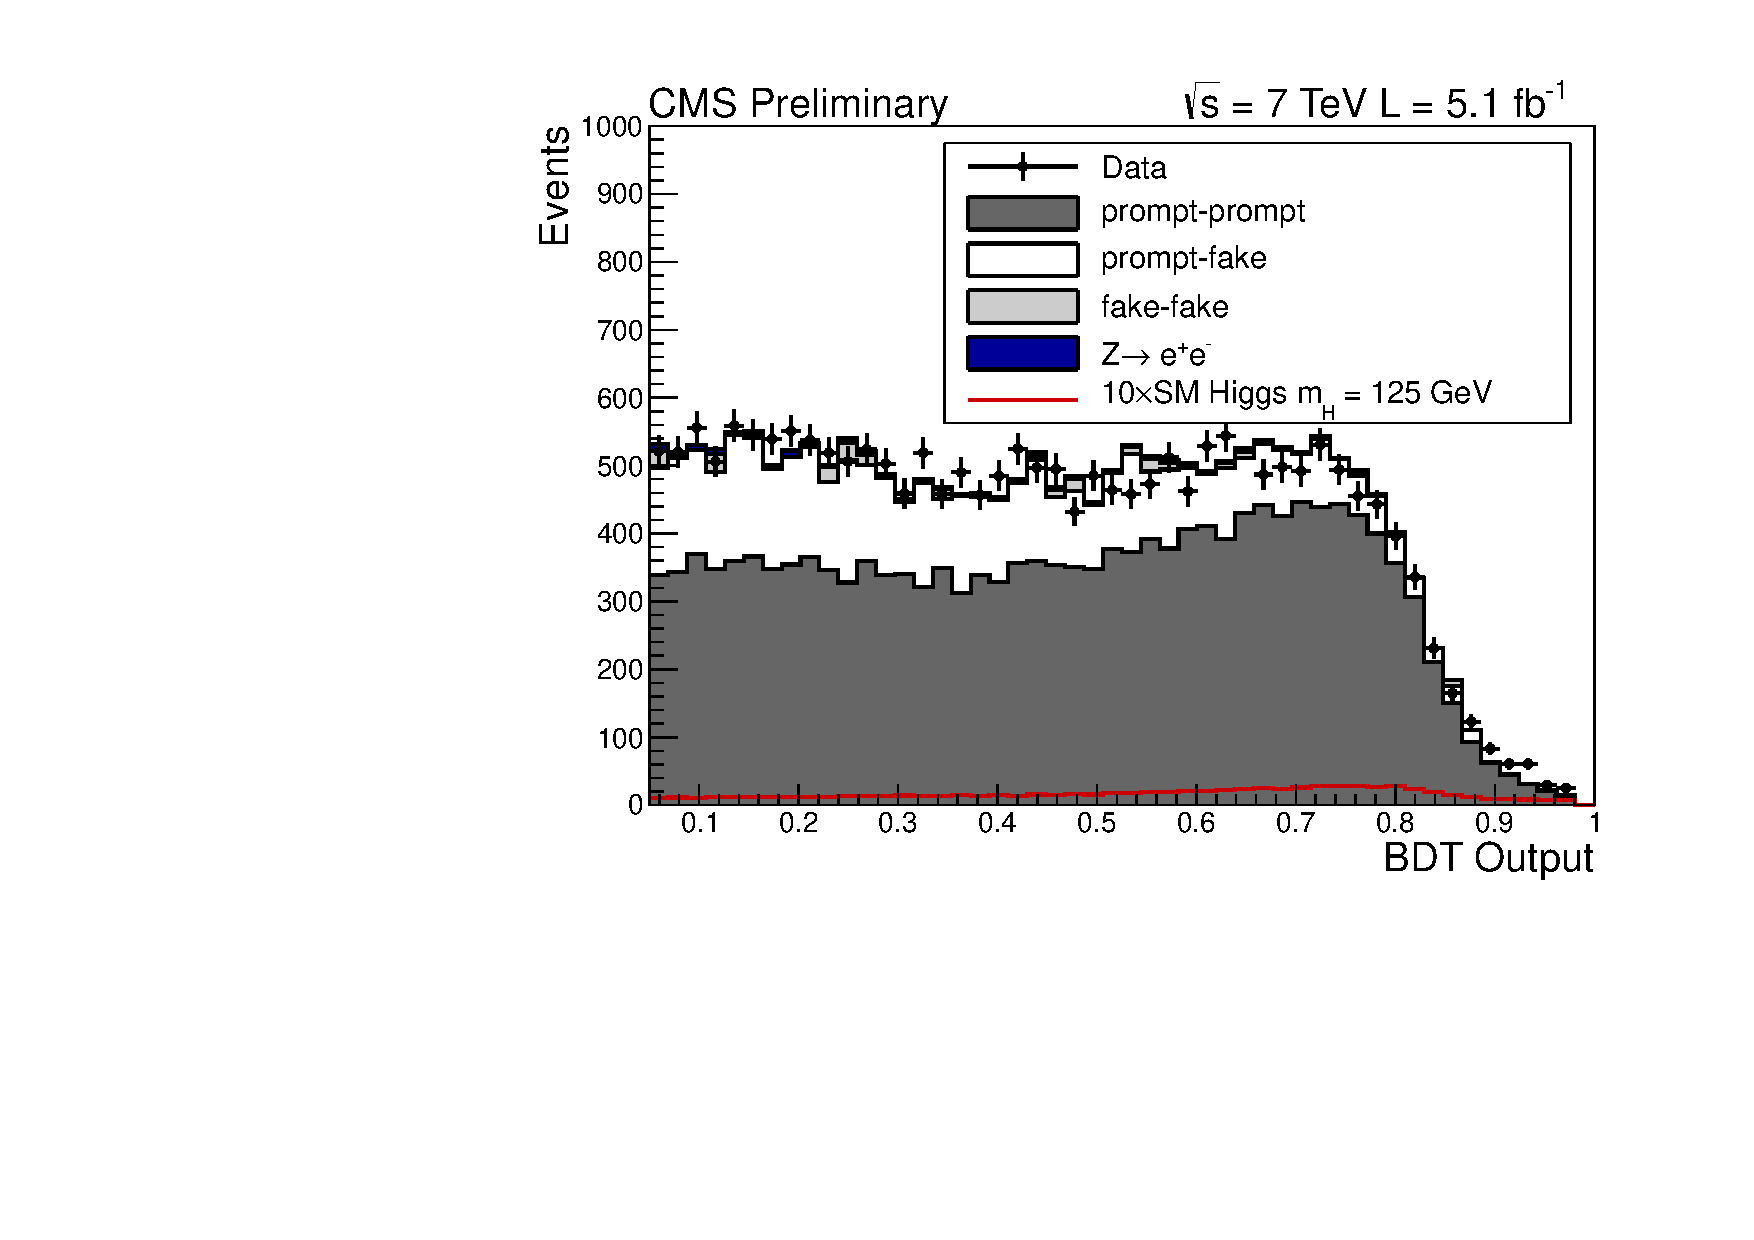
\includegraphics[width=0.8\textwidth]{hgg7TeV/variablePlots/bdtoutput}
 \caption{Diphoton BDT distribution in data and MC. The contribution expected from a SM Higgs boson with mass 125 GeV, 
 scaled by 100, is shown in red. }
 \label{fig:diphotonBDT}
\end{figure}
\begin{figure}[hbt!]
  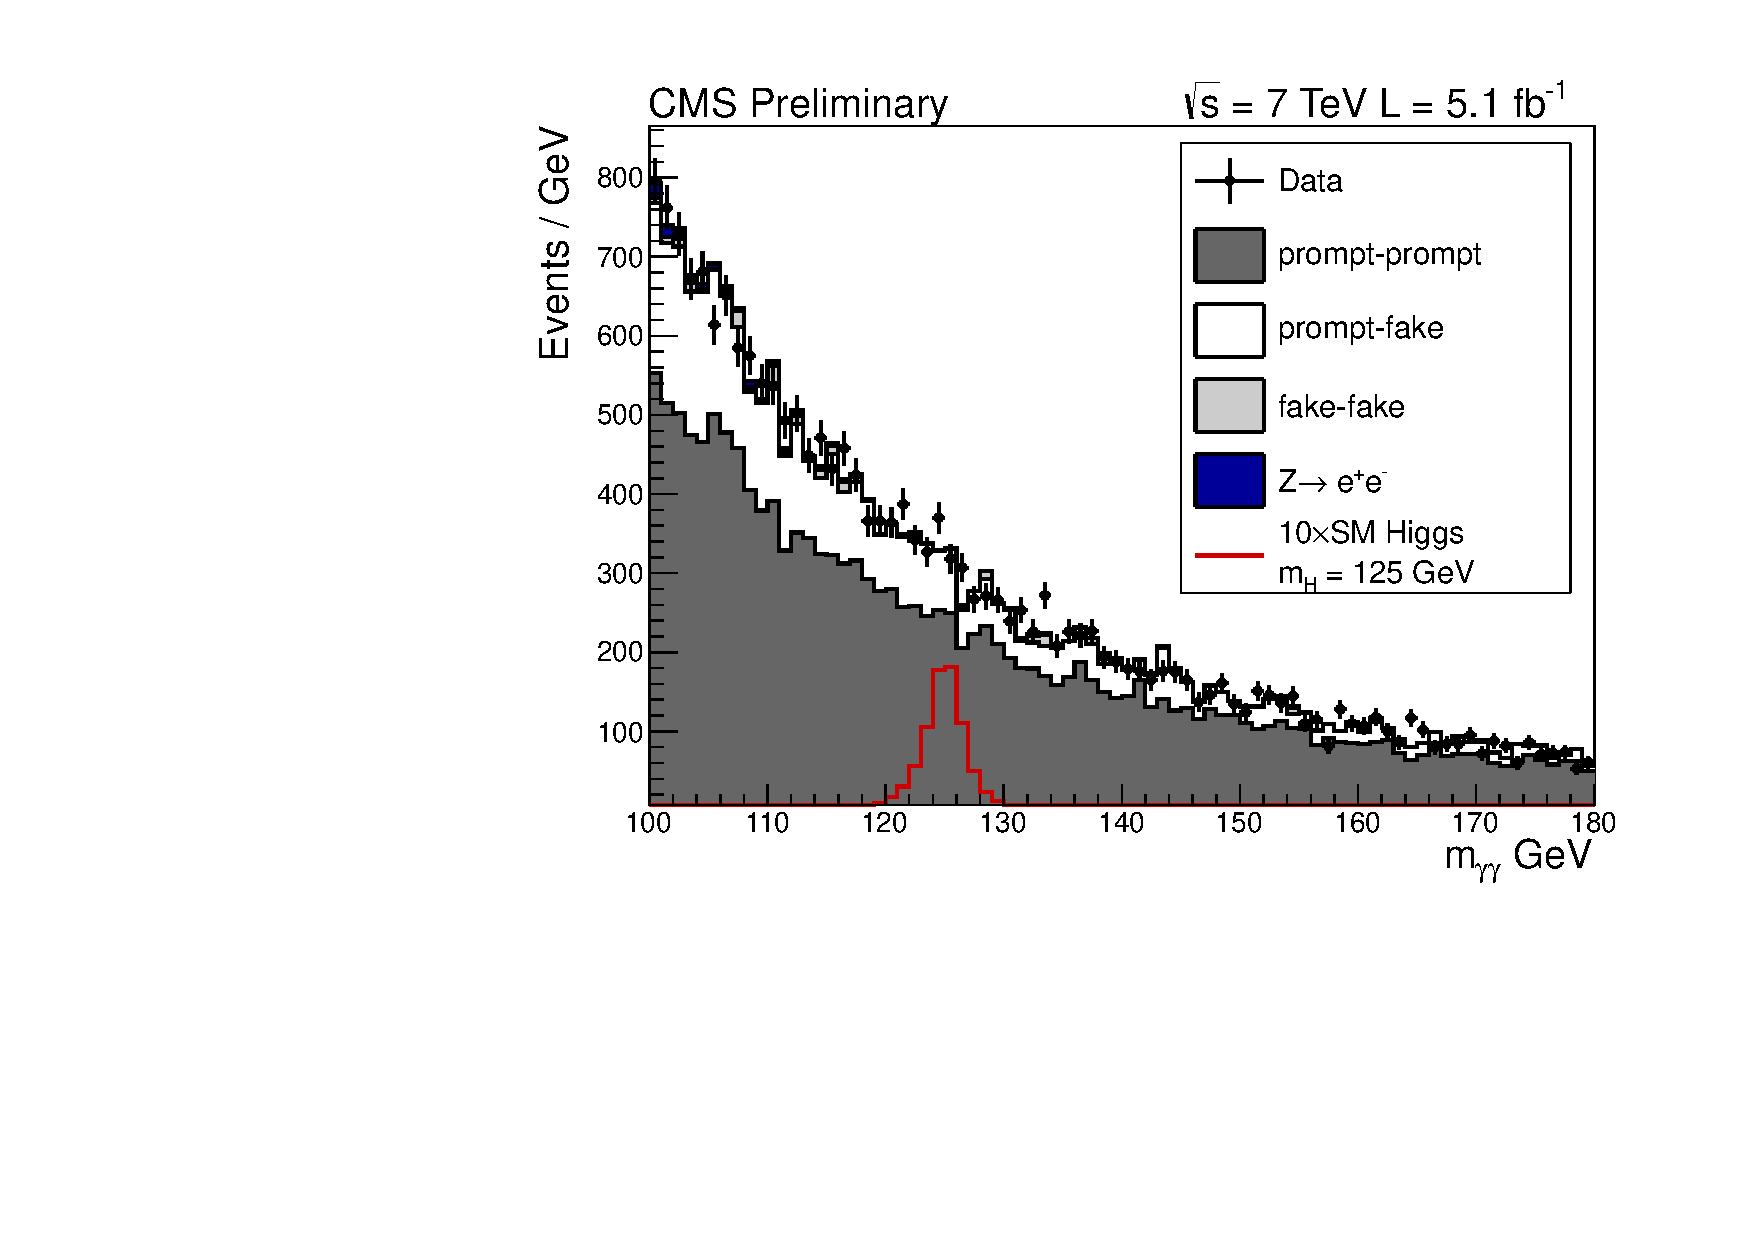
\includegraphics[width=0.8\textwidth]{hgg7TeV/variablePlots/mass}
 \caption{Invariant mass distribution in data and MC after applying the full event selection in the
 range 100 to 180 GeV. The contribution expected from a SM Higgs boson with mass 125 GeV, scaled by 10, 
 is shown in red. }
 \label{fig:massmcdata}
\end{figure}

\subsubsection{Diphoton BDT Validation with $\Zee$ Data}
By using a BDT for the full event selection, subtle correlations between the input variables are accounted for
which improve the separation between the signal and background. 
Unlike the background model, the signal model is derived from corrected MC. 
It is important therefore to ensure that the BDT will respond in the same way in data as for the signal MC
used for the signal extraction. The MC can be validated using $\Zee$ data-MC
comparisons by inverting the electron veto and treating the electrons as though they were photons.
This is done by using the supercluster associated to the electron for the electron's energy measurement 
and ignoring the track information. In this way, the reconstruction of the electrons is the same as that
of the photons allowing for validation of the BDT's response to real photons from a resonant decay. 
Figure~\ref{fig:zeevaliddiphomva} shows the diphoton BDT distribution in $\Zee$ MC and data after applying
the full selection using this technique. The discrepancies between MC and data are well covered by the 
systematic uncertainties on the photon ID BDT output and $\sigma_{E}$ which are included in the final signal model. 

\begin{figure}
  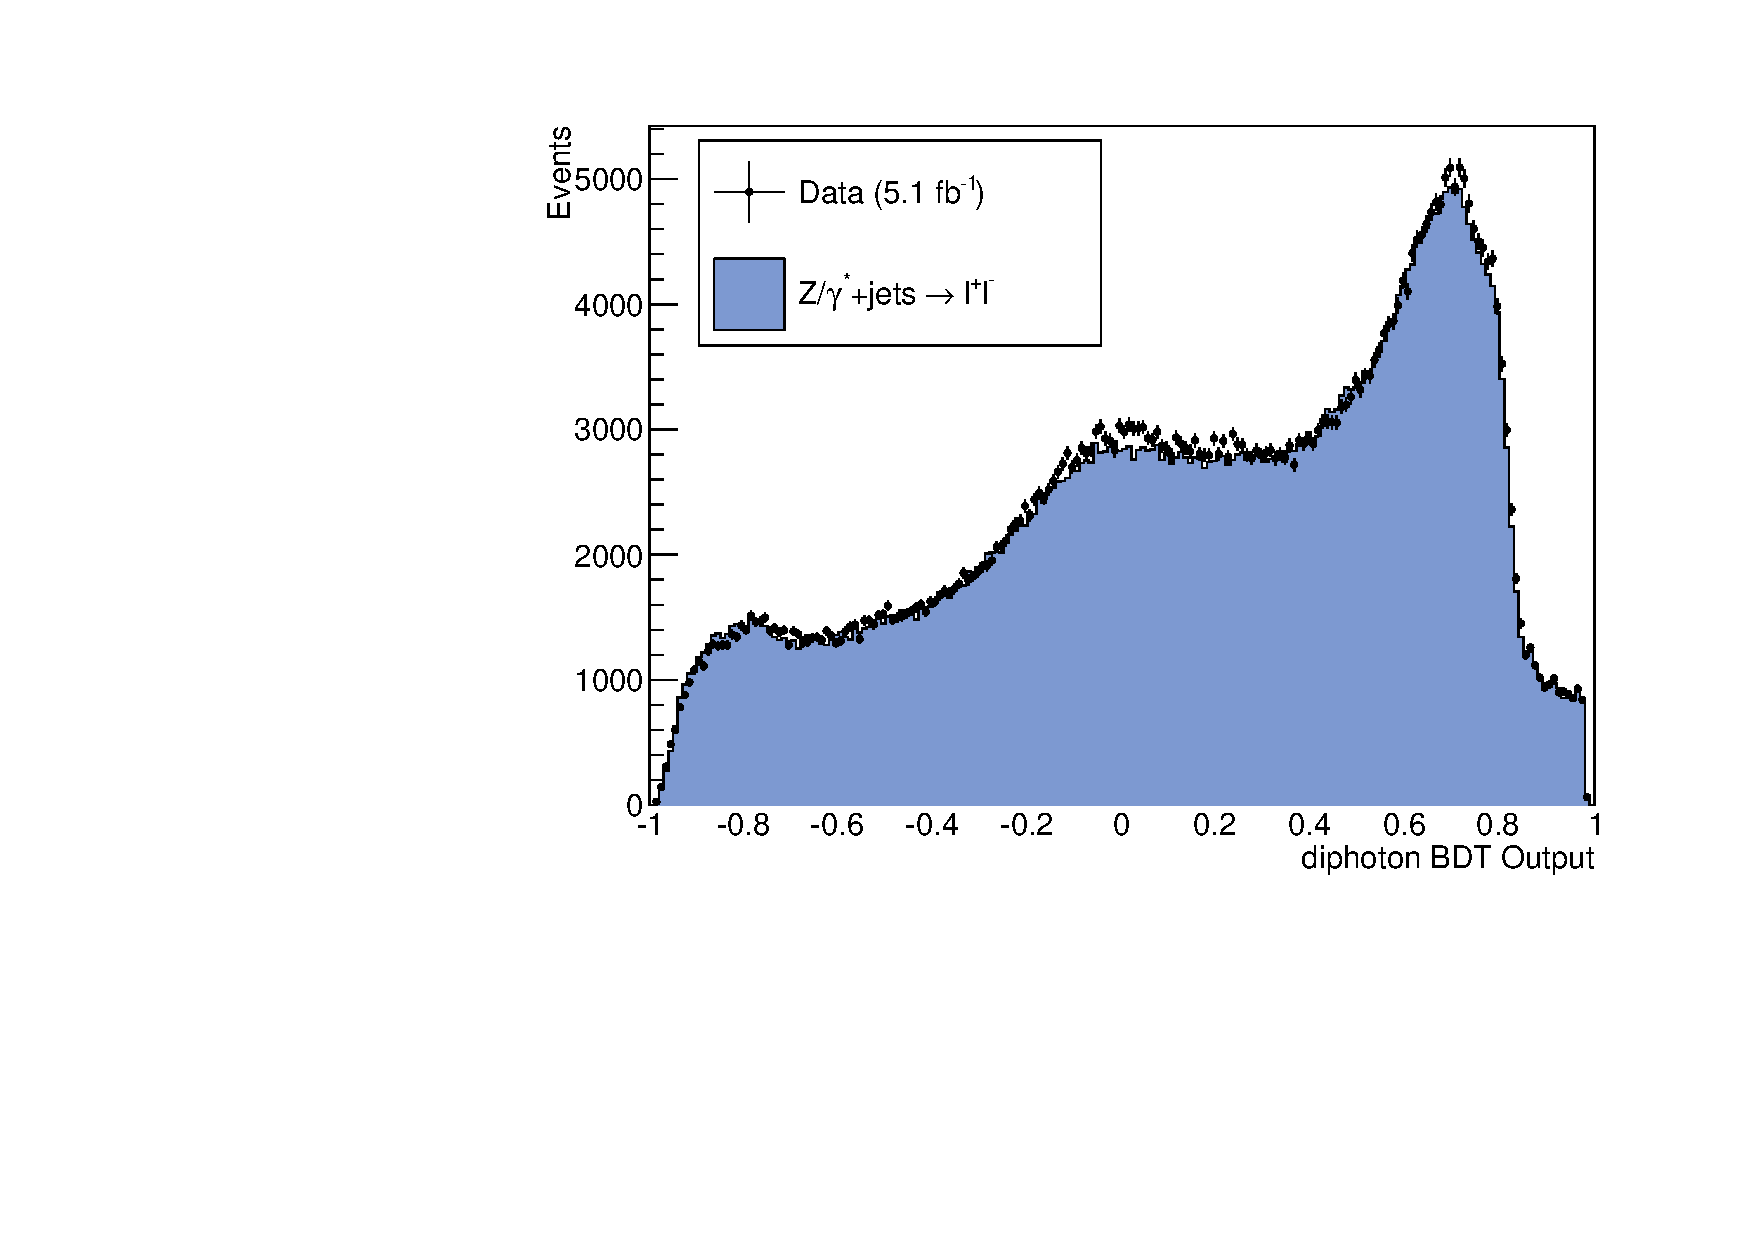
\includegraphics[width=.8\textwidth]{hgg7TeV/zeeValidation/zeevalidationdipho.pdf}\\
  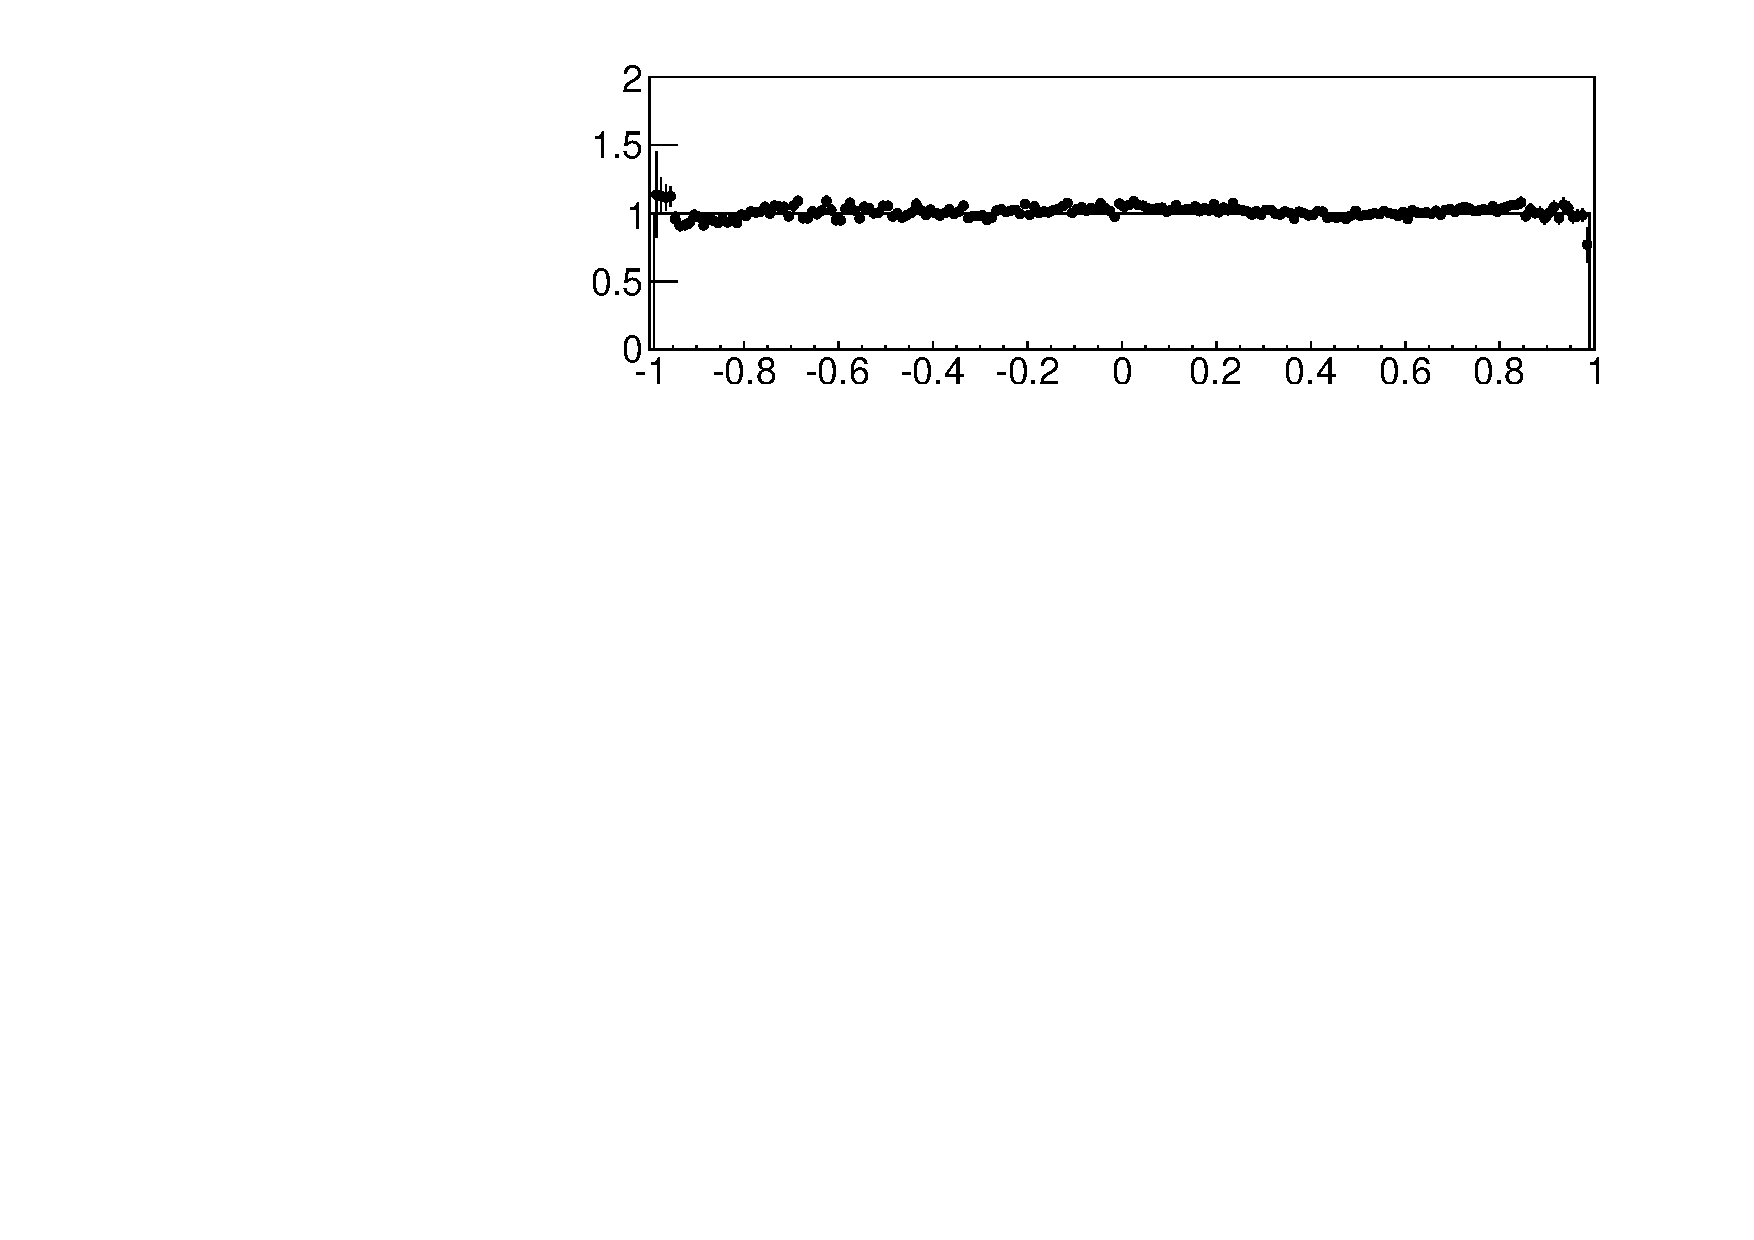
\includegraphics[width=.8\textwidth]{hgg7TeV/zeeValidation/zeevalidationdipho_ratio.pdf}
\caption{Diphoton BDT output distribution in $\Zee$ MC and data after the full selection 
treating the electrons as photons for the purposes of energy reconstruction. The electron 
veto is inverted to preferentially select electrons. The lower panel show the data/MC ratio.}
\label{fig:zeevaliddiphomva}
\end{figure}

Both the photon ID and regression BDT rely on a detailed simulation of electromagnetic showering  
in MC to correctly describe the data. Due to imperfections of this simulation, systematic
uncertainties are included in the signal model to cover the residual difference observed between MC and data
for high $\pt$ photons. 
These uncertainties are validated using $\Zee$ data in the same way as the diphoton BDT. 
Figures~\ref{fig:zeevalidsigmaE} and~\ref{fig:zeevalidphoidmva} show the distributions of the 
per photon energy resolution estimator $\sigma_{E}$ relative to the photon energy and the output of the 
photon ID BDT in $\Zee$ MC and data treating the electrons as photons. The red lines
show the $\pm 1\sigma$ error envelope attributed to the systematic uncertainty on the shower simulation.  
These uncertainties are propagated through the diphoton BDT and included in the signal model as described in 
Section~\ref{sec:signalmodel}.

\begin{figure}
  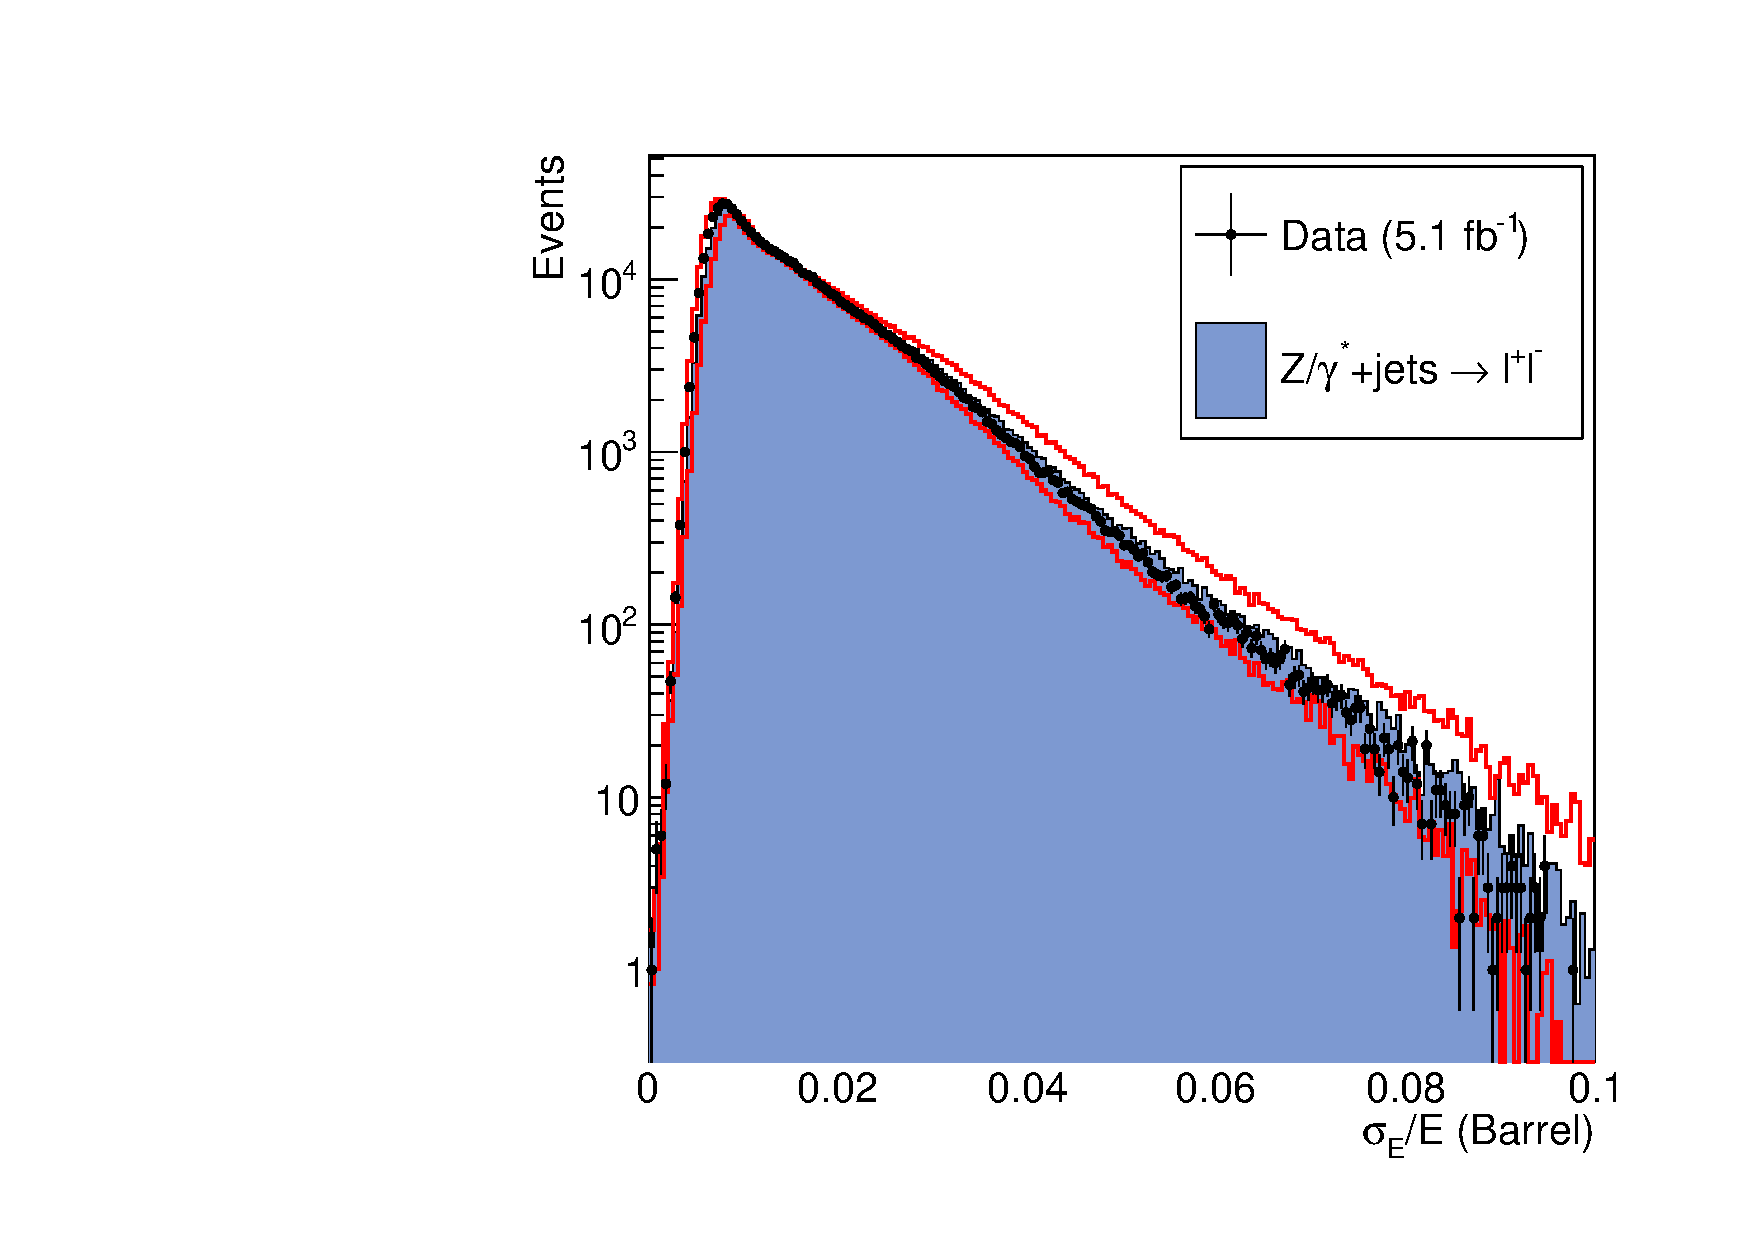
\includegraphics[width=.48\textwidth]{hgg7TeV/zeeValidation/sigmaE_EB.pdf}
  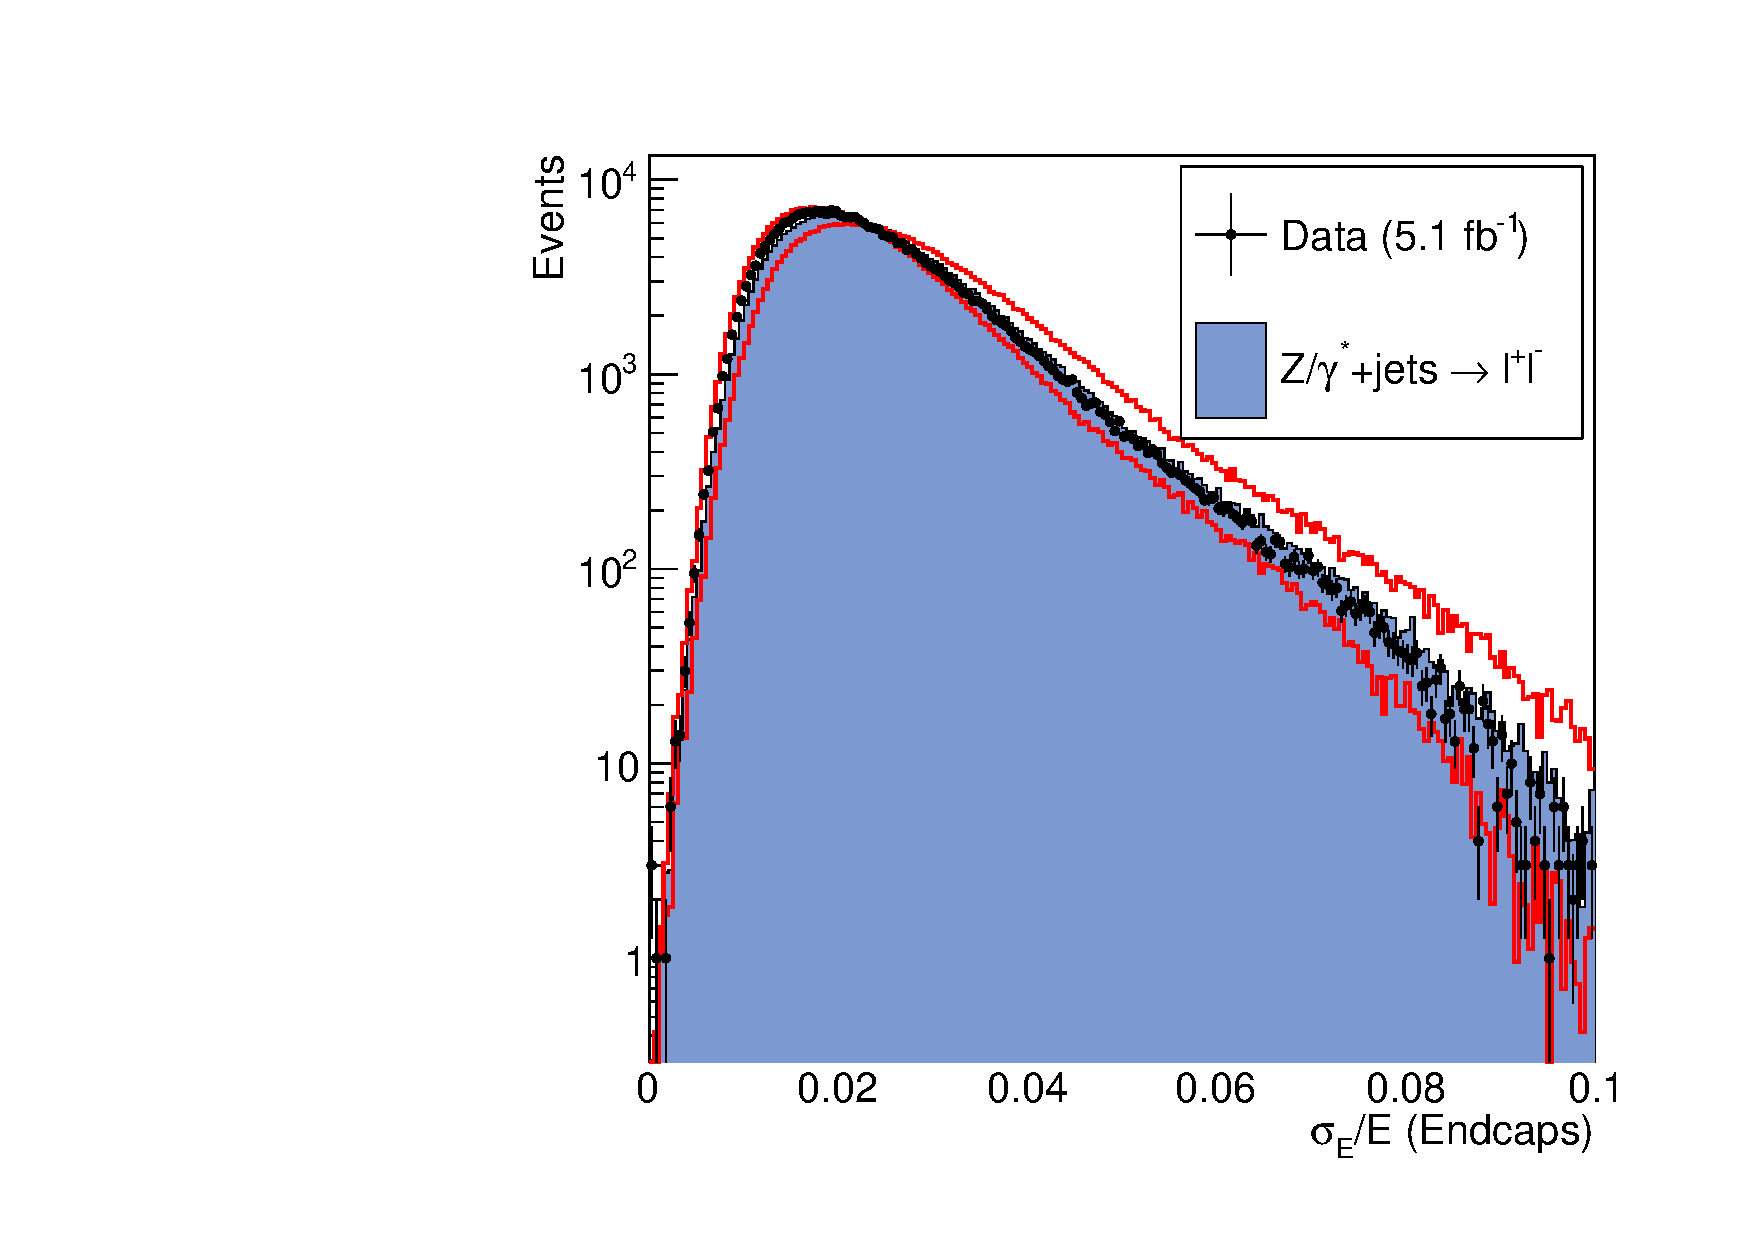
\includegraphics[width=.48\textwidth]{hgg7TeV/zeeValidation/sigmaE_EE.pdf}\\
  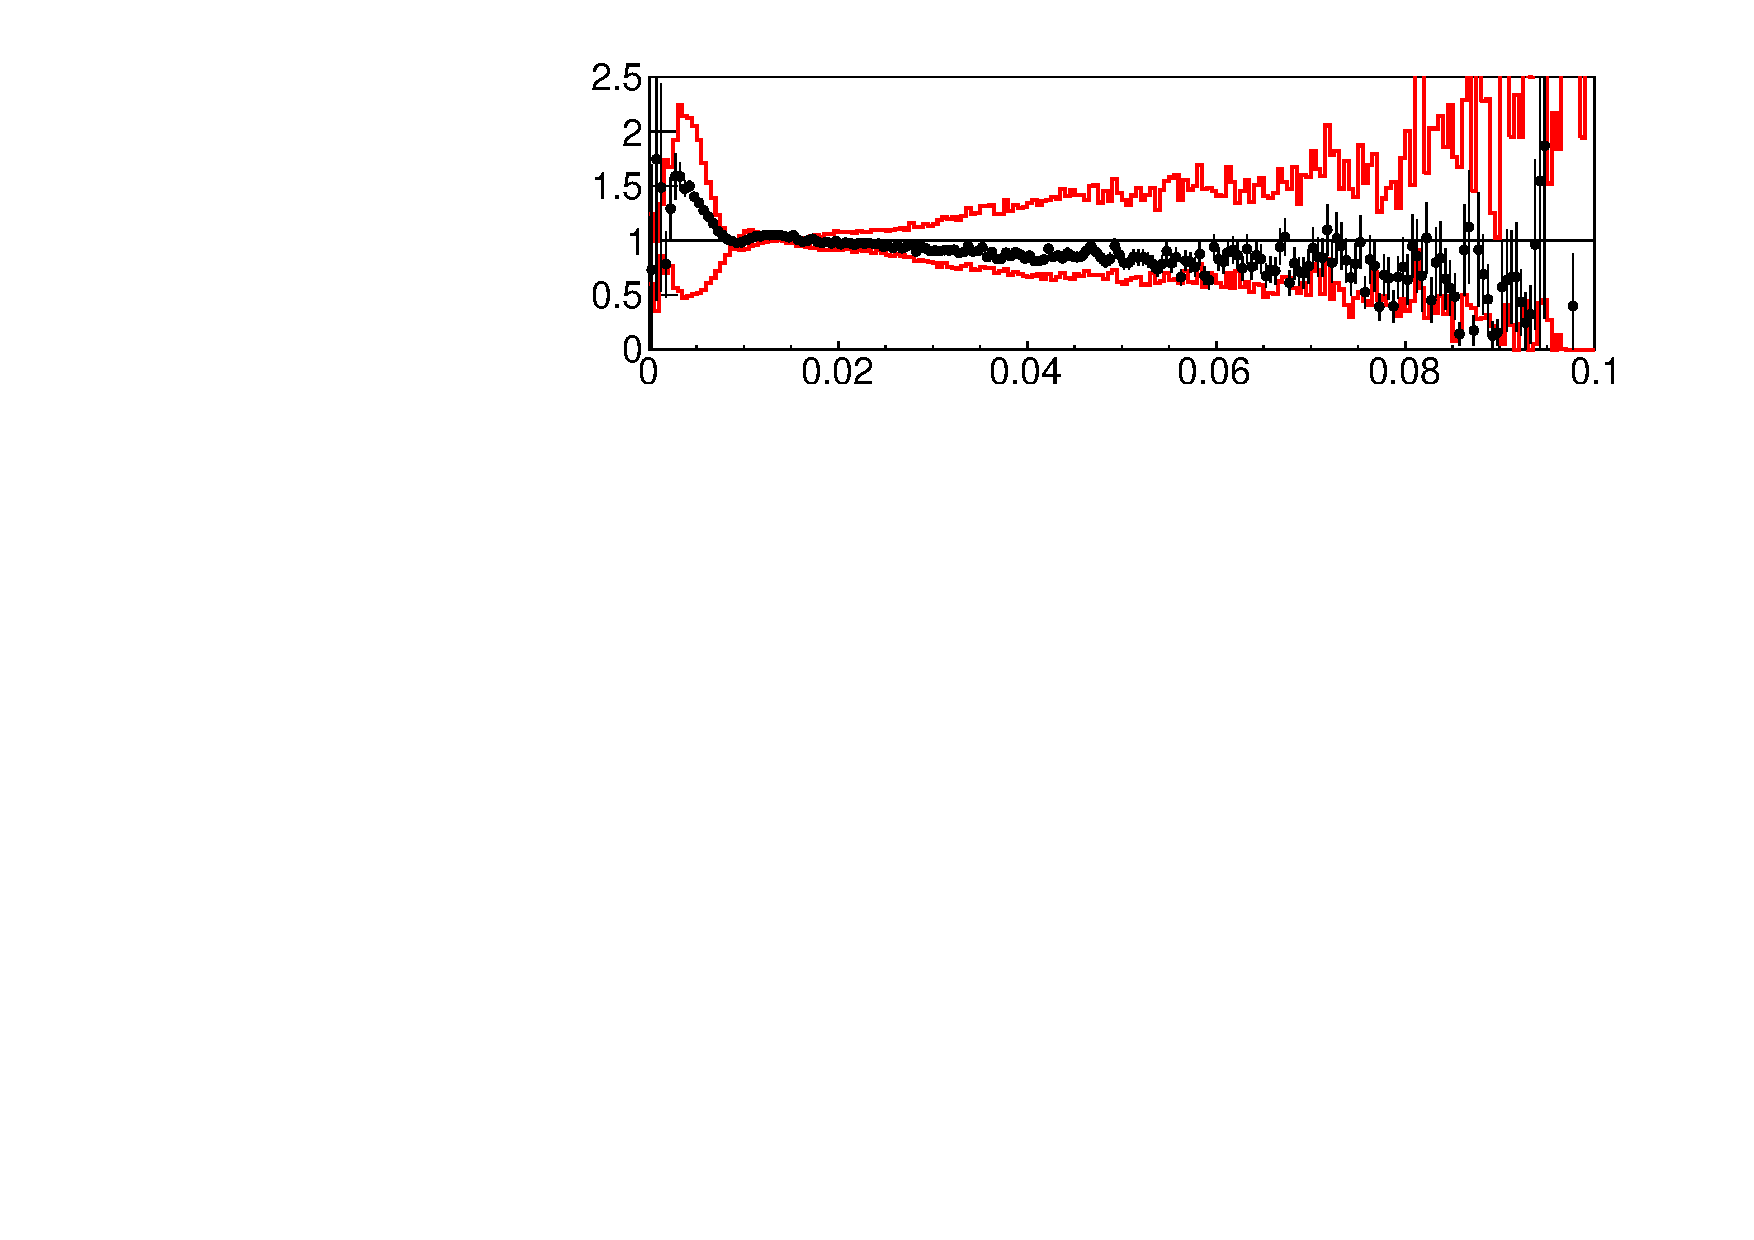
\includegraphics[width=.48\textwidth]{hgg7TeV/zeeValidation/sigmaE_EB_ratio.pdf}
  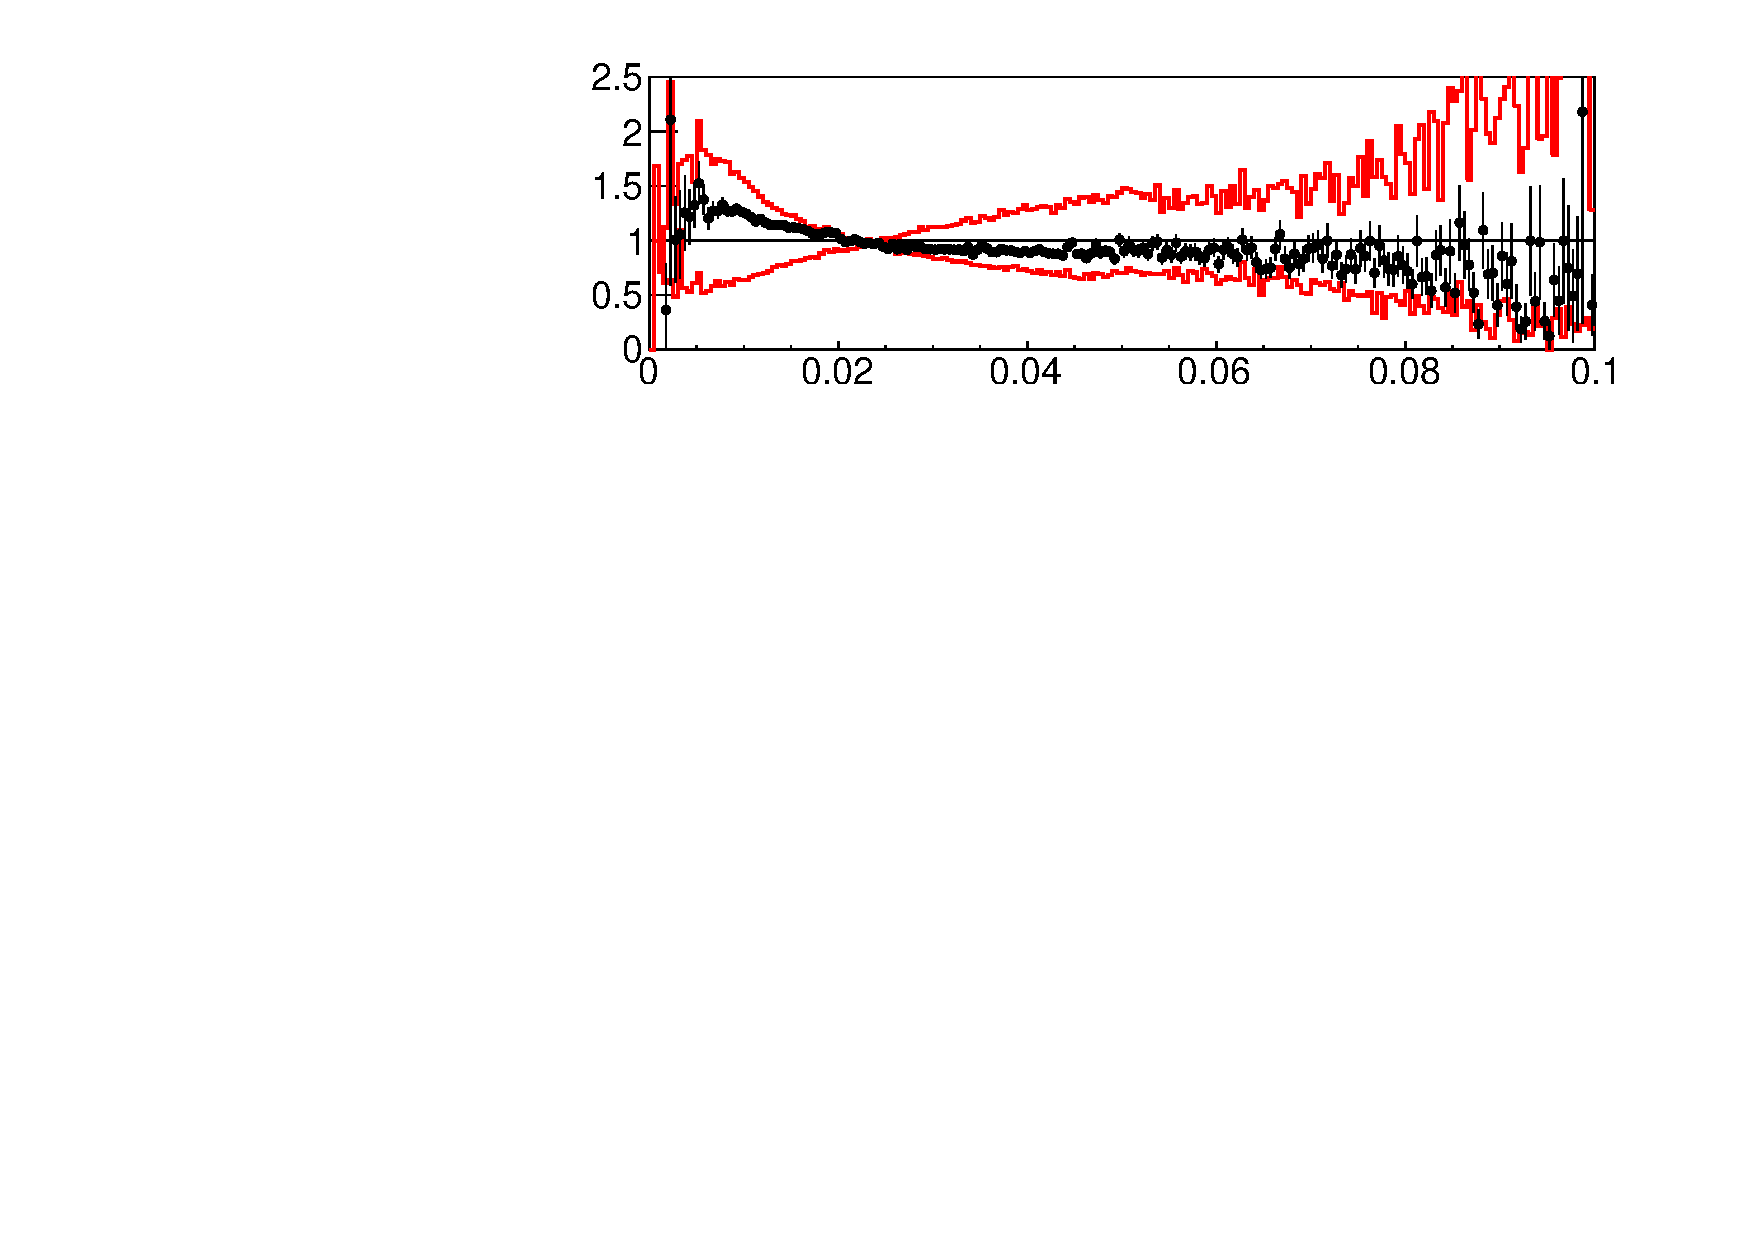
\includegraphics[width=.48\textwidth]{hgg7TeV/zeeValidation/sigmaE_EE_ratio.pdf}
\caption{Per-photon resolution estimator, $\sigma_{E}$, relative to the measured energy in $\Zee$ 
MC and data 
treating the electrons as photons in the barrel (left) and endcaps (right). 
The red lines show the $\pm 1\sigma$ systematic error envelope obtained by scaling the value of 
$\sigma_{E}$ by $\pm 10\%$. The lower panels show the ratios to the nominal MC distributions.}
\label{fig:zeevalidsigmaE}
\end{figure}

\begin{figure}
  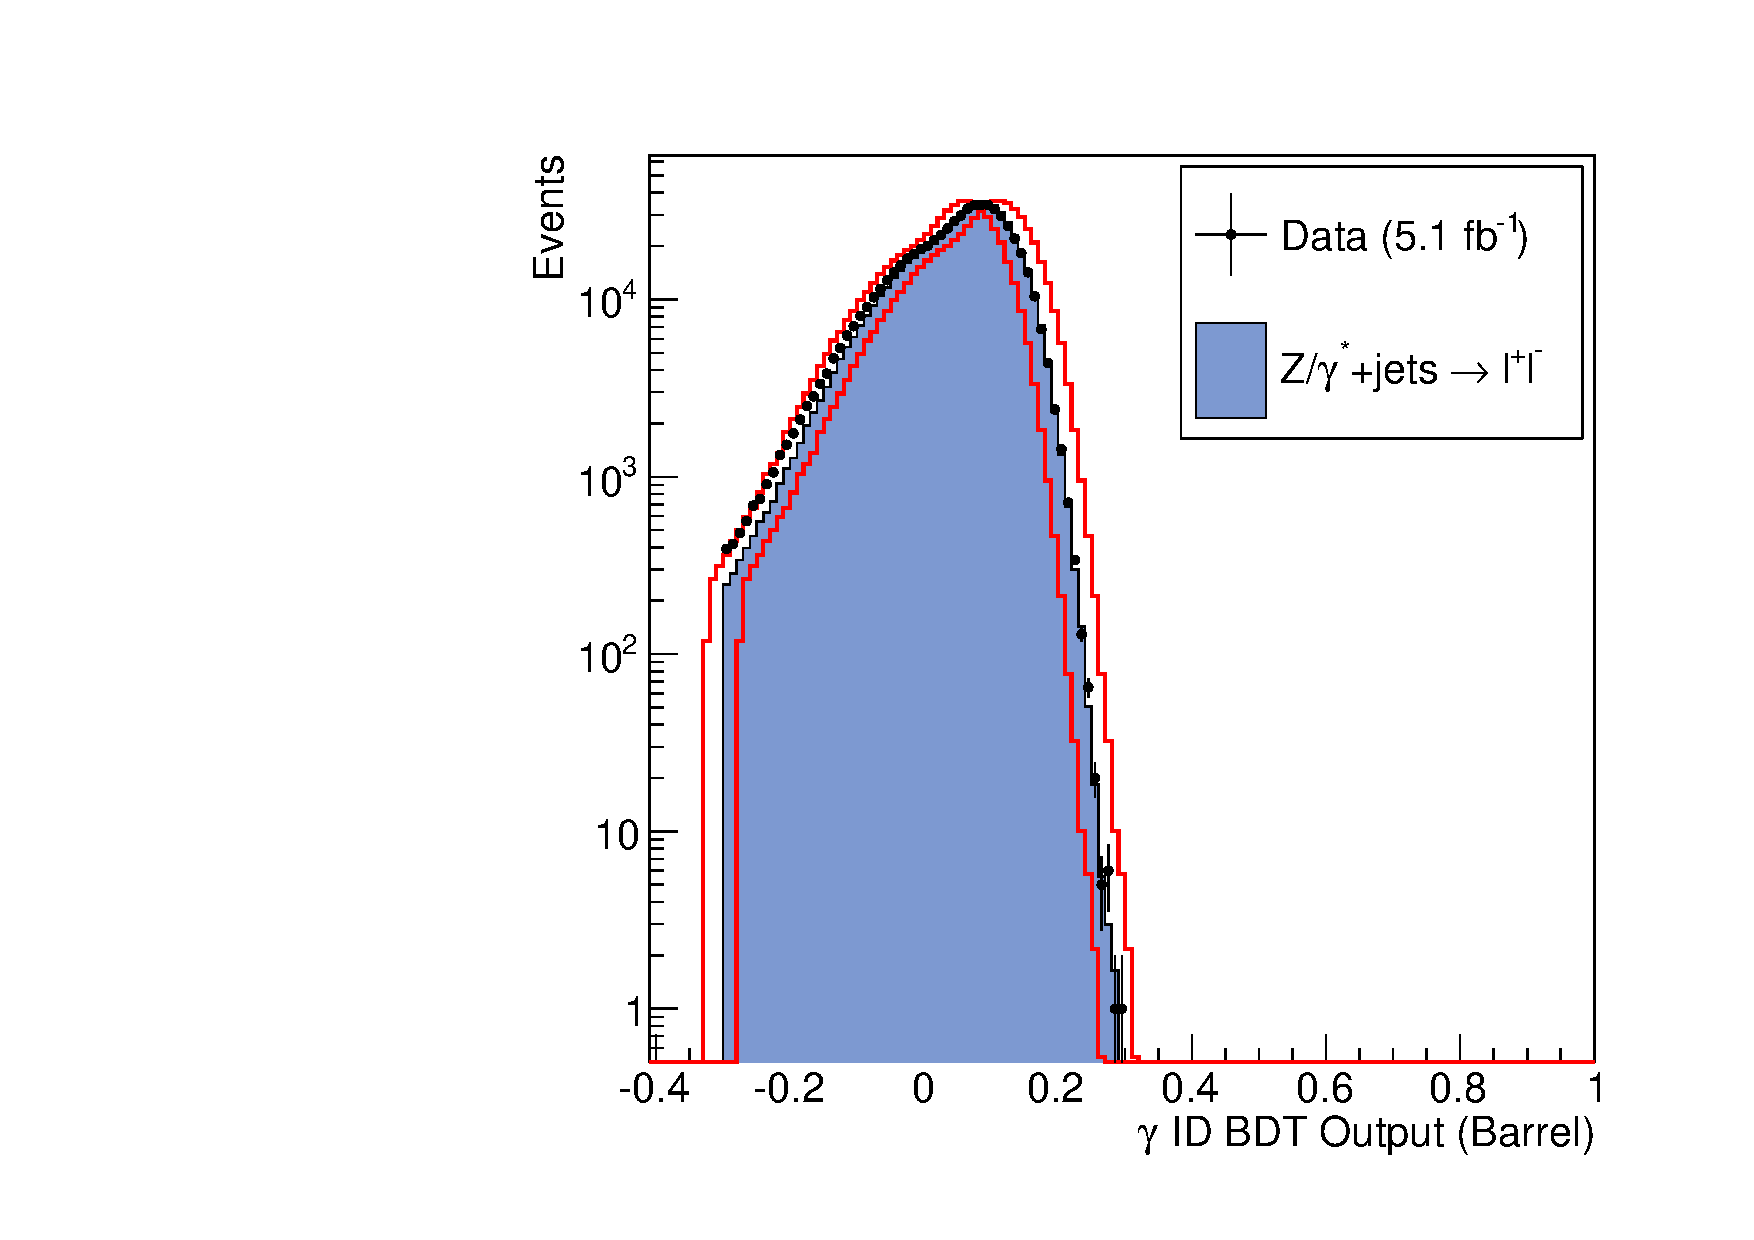
\includegraphics[width=.48\textwidth]{hgg7TeV/zeeValidation/phoID_EB.pdf}
  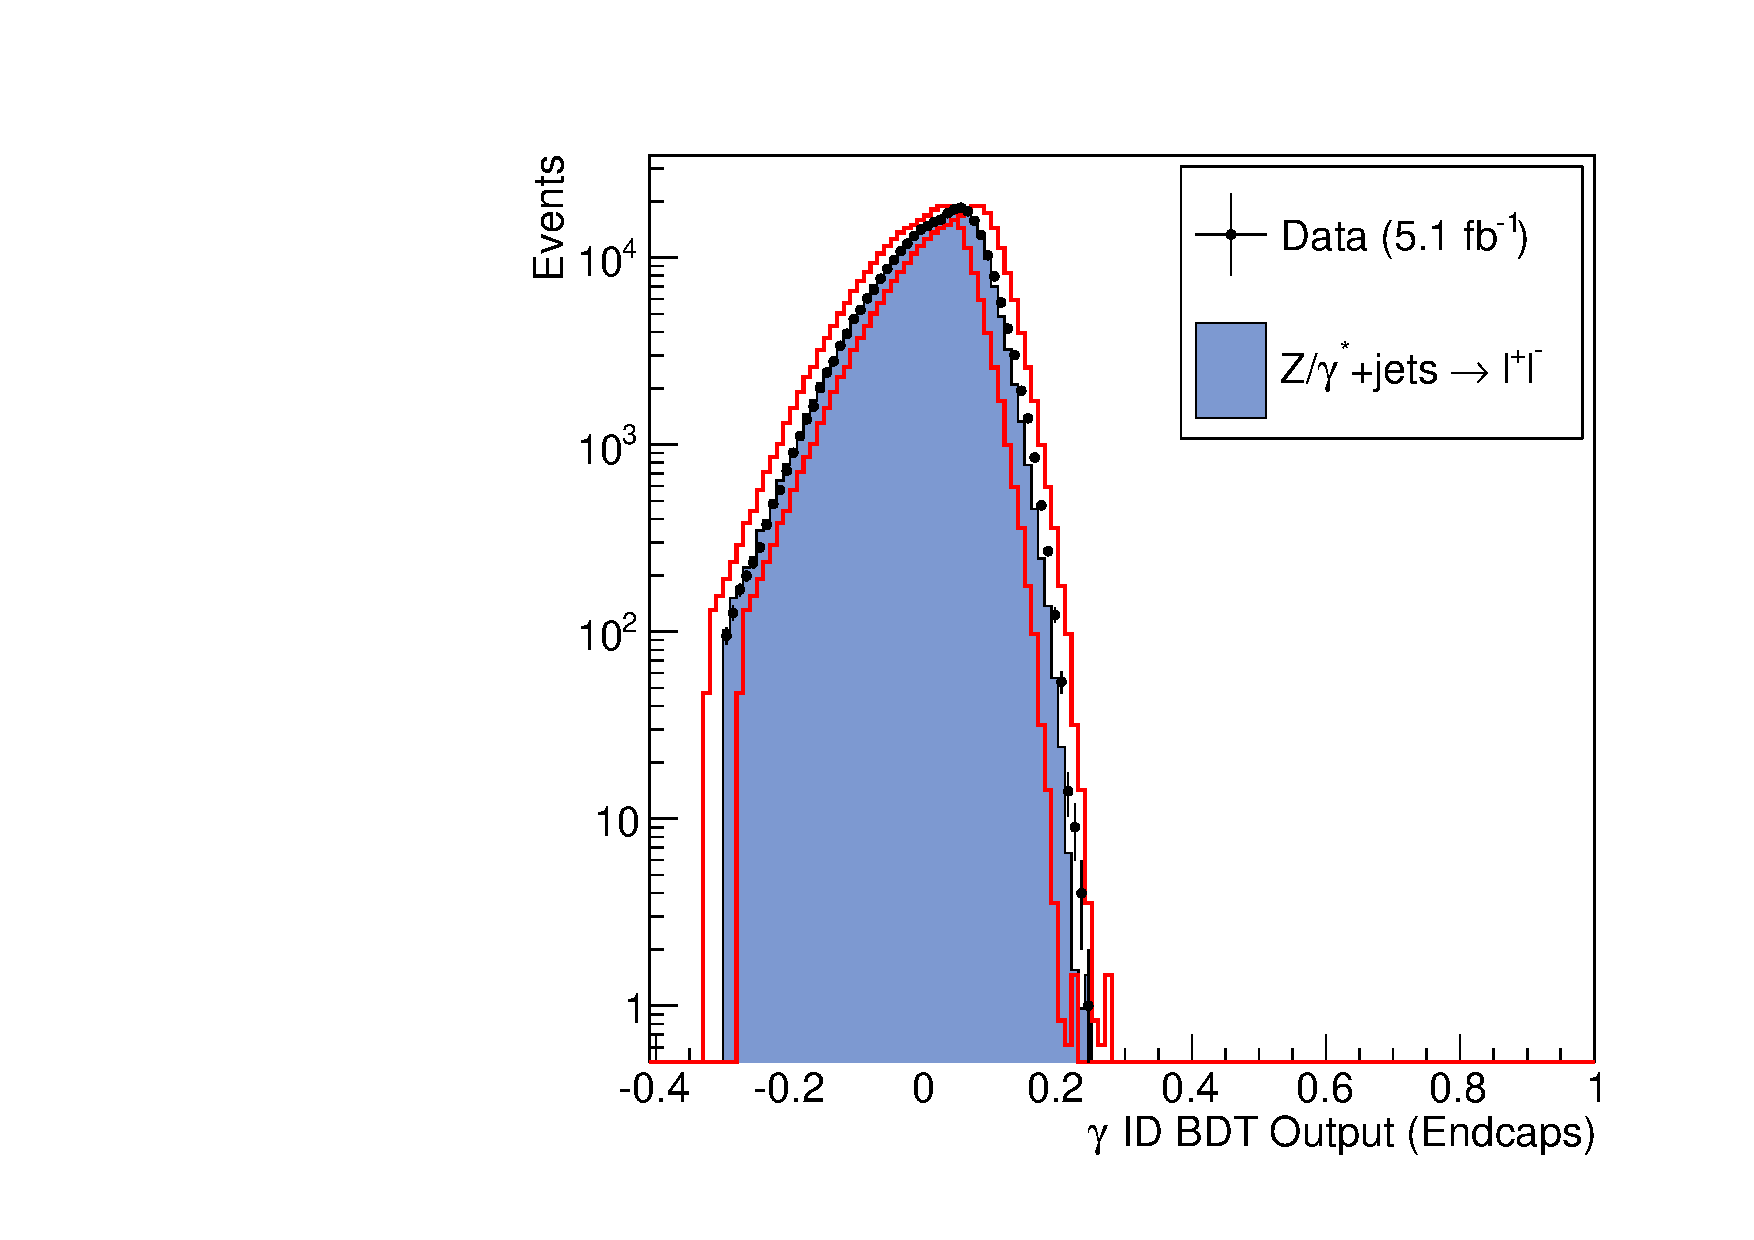
\includegraphics[width=.48\textwidth]{hgg7TeV/zeeValidation/phoID_EE.pdf}\\
  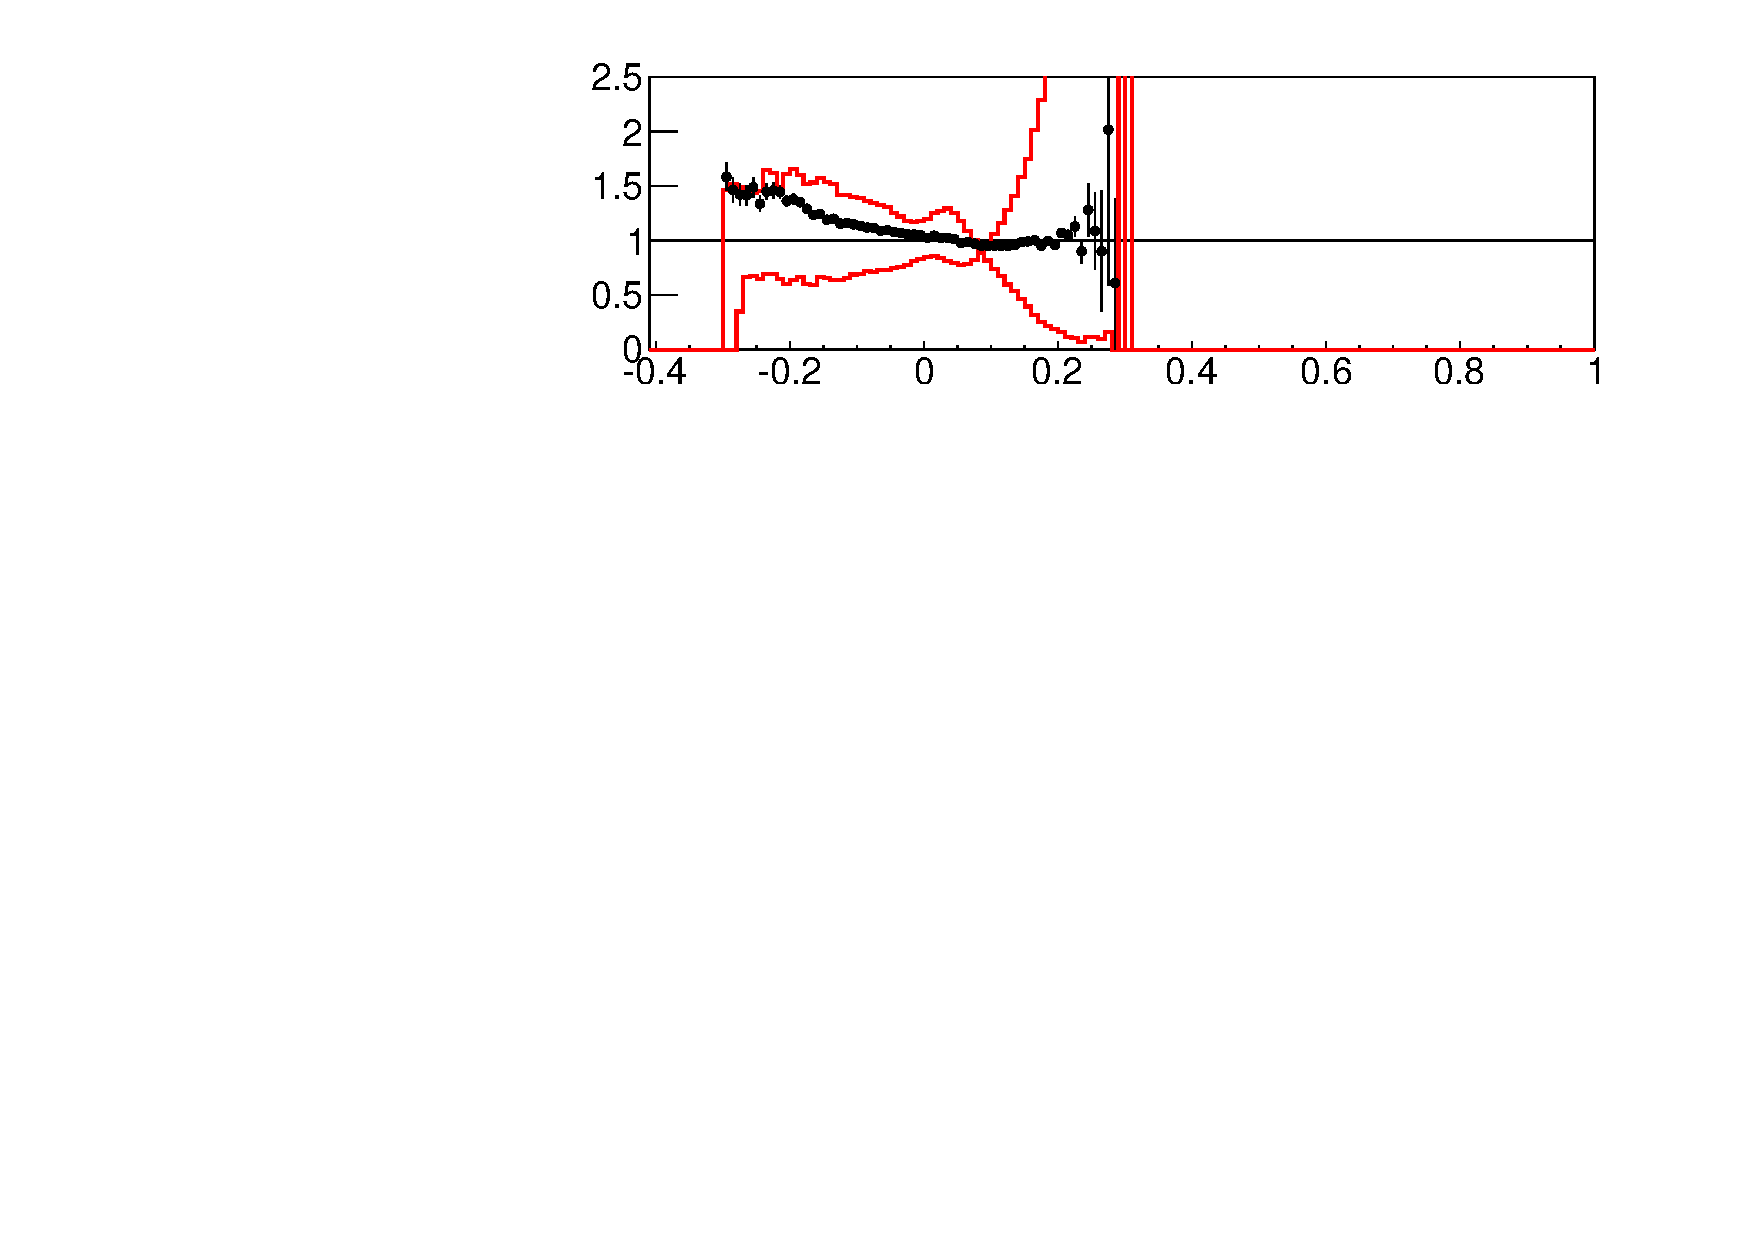
\includegraphics[width=.48\textwidth]{hgg7TeV/zeeValidation/phoID_EB_ratio.pdf}
  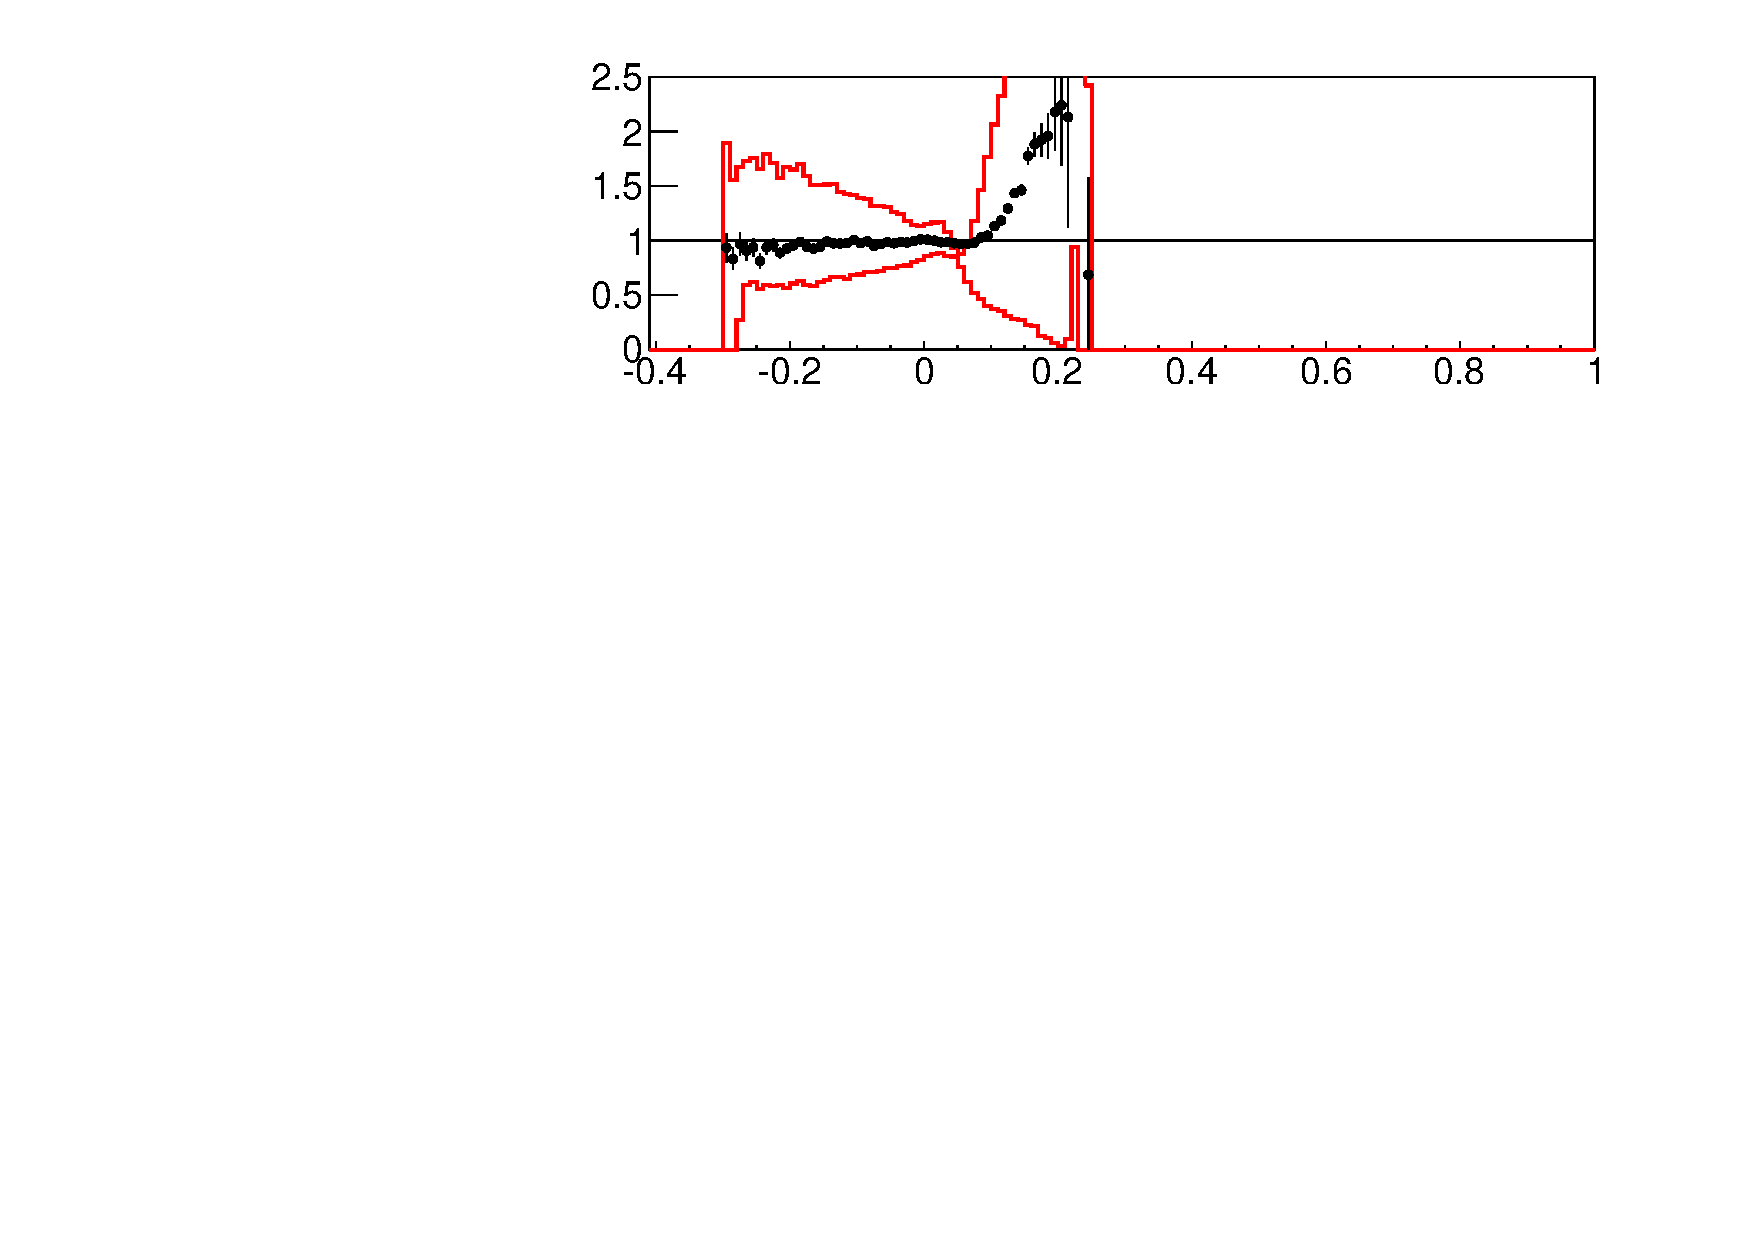
\includegraphics[width=.48\textwidth]{hgg7TeV/zeeValidation/phoID_EE_ratio.pdf}\\
\caption{Photon ID BDT output in $\Zee$ MC and data 
treating the electrons as photons in the barrel (left) and endcaps (right). 
The red lines show the $\pm 1\sigma$ systematic error envelope obtained by shifting the output value by $\pm 0.025\%$.
The lower panels show the ratios to the nominal MC distributions.}
\label{fig:zeevalidphoidmva}
\end{figure}

\subsection{Dijet Tagging}
\label{sec:dijettagging}

The contribution to Higgs boson production from vector boson fusion is around a factor ten smaller than that
of gluon-gluon fusion. However, additional information from the two jets associated 
with $qqH$ production allows further reduction of the diphoton background~\citep{HIG-11-033}.
Events containing two jets which pass the full selection and in addition
satisfy a series of criteria designed to target the specific dijet topology are 
tagged as likely to have originated from $qqH$ production. For example, Figure~\ref{fig:vbfdeta} shows the 
separation in $\eta$ between the two jets. Signal events from vector boson fusion production are
more likely to have a large separation than those from background processes. The full set of 
criteria is given in Table~\ref{tab:vbfcuts}.
The dijet tagged events are categorized separately to 
the remaining events, thereby exploiting their high signal to background ratio for the purpose of signal
extraction. 

\begin{table}
\begin{tabular*}{0.5\textwidth}{@{\extracolsep{\fill}}|l|c|}
\hline
\textbf{Variable} & \textbf{Cut Value} \\
\hline
\hline
$E_{T}^{j^{1}}$ & $>$ 30 GeV \\
$E_{T}^{j^{2}}$ & $>$ 20 GeV \\
$m_{jj}$ 	 & $>$ 350 GeV \\
$|\eta_{j^{1}} - \eta_{j^{2}}|$ & $>$ 3.5 \\
$|\phi_{jj} - \phi_{\gamma\gamma}|$ & $>$ 2.6 \\
$|\frac{1}{2}(\eta_{j^{1}} + \eta_{j^{2}}) - \eta_{\gamma\gamma}|$ & $<$ 2.5 \\
\hline
\end{tabular*}
\caption{Dijet selection criteria for the two $qqH$ jets. The leading and sub-leading $E_{T}$ jets
are denoted $j^{1}$ and $j^{2}$ respectively.}
\label{tab:vbfcuts}
\end{table}

\begin{figure}
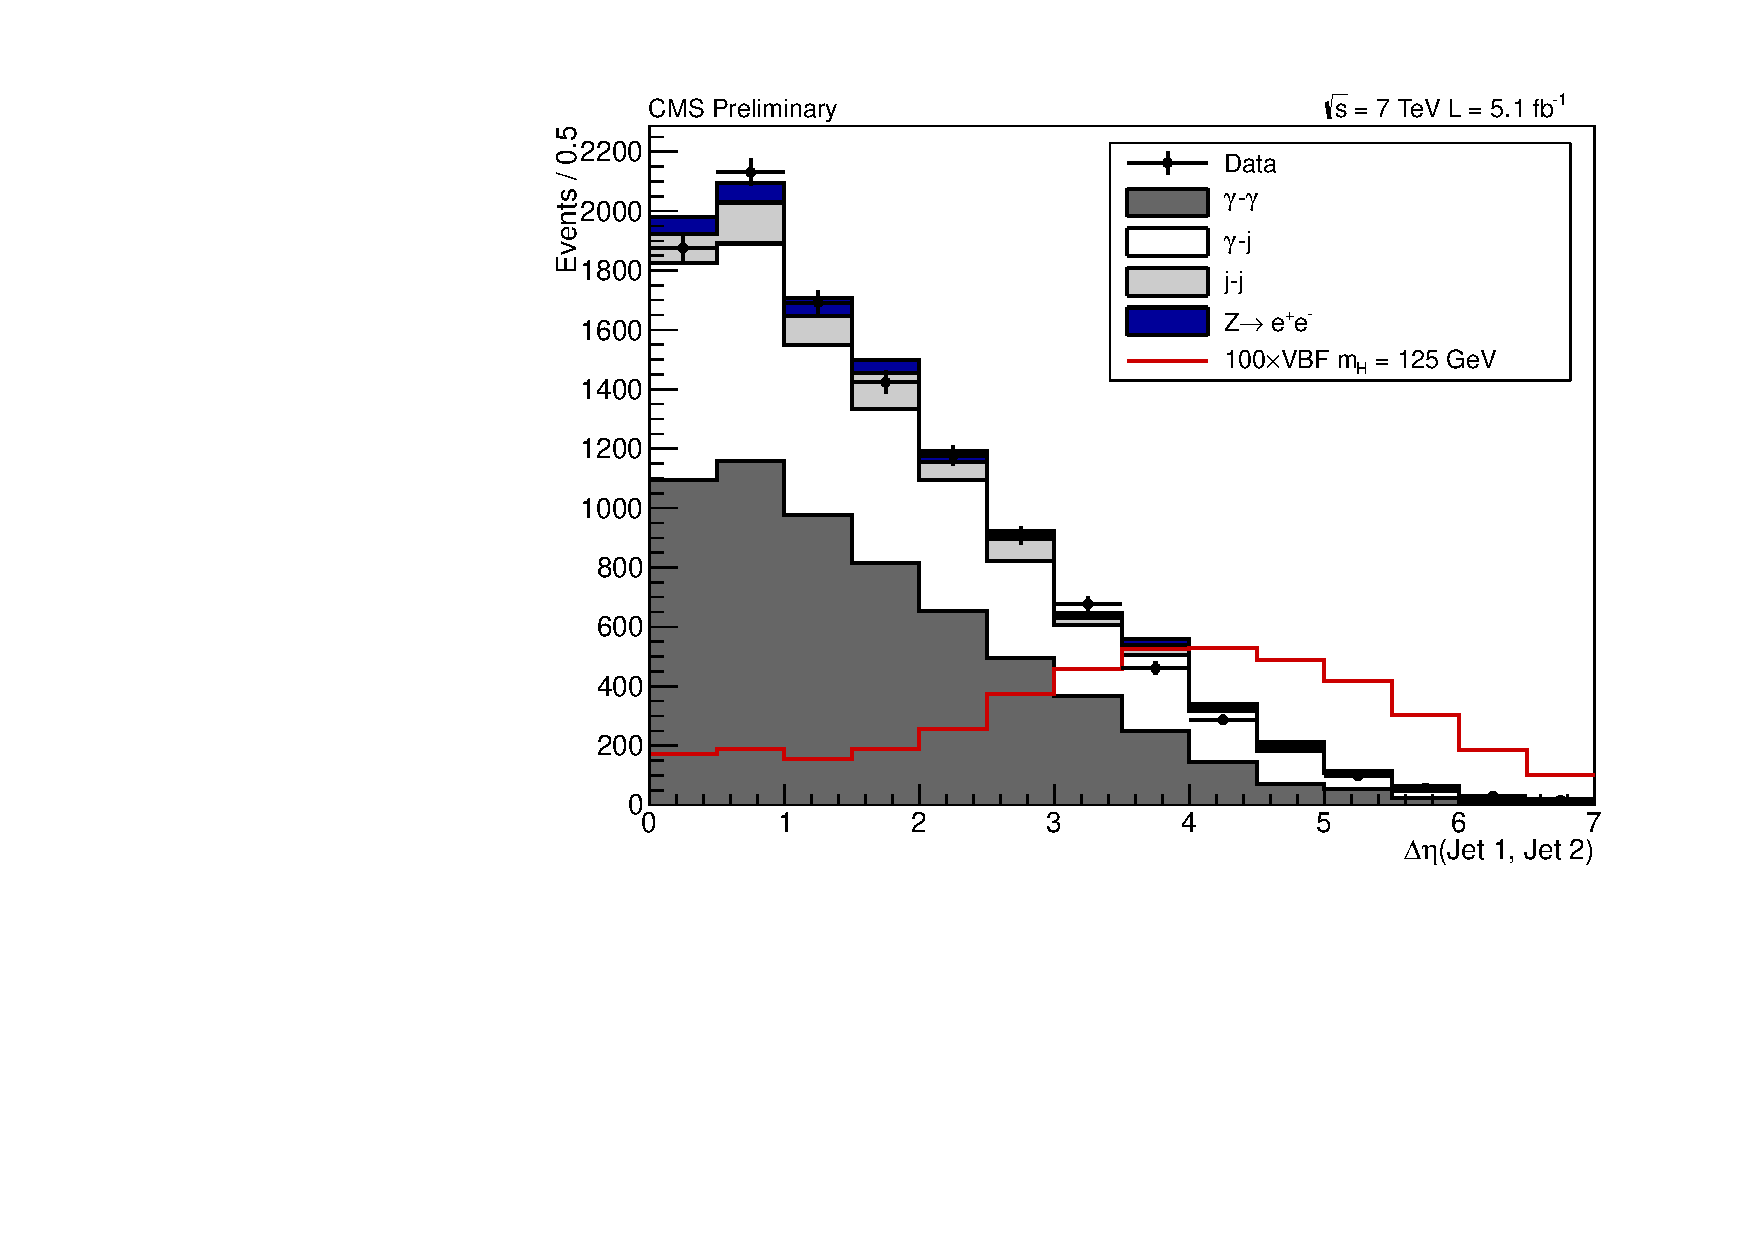
\includegraphics[width=0.8\textwidth]{hgg7TeV/variablePlots/cut_VBF_dEta_sequential_cat0.pdf}
\caption{Separation in $\eta$ between two identified jets in data and MC. 
The expectation from a SM Higgs boson produced via vector boson fusion ($qqH$), scaled by 100,
is shown in red. All cuts other than the one on $\Delta\eta(Jet 1, Jet2)$ are applied to these distributions.} 
\label{fig:vbfdeta}
\end{figure}

